\documentclass[11pt,a4paper]{article}
\usepackage[a4paper,margin=2.1cm]{geometry}
\usepackage[T1]{fontenc}
\usepackage{newtxtext,newtxmath}
\usepackage{microtype}
\usepackage{graphicx}
\usepackage{booktabs}
\usepackage[table]{xcolor}
\usepackage{amsmath}
\usepackage{caption}
\usepackage{subcaption}
\usepackage{enumitem}
\usepackage{multirow}
\usepackage{float}
\usepackage{needspace}
\usepackage{placeins}
\usepackage[round]{natbib}
\usepackage[colorlinks=true,linkcolor=blue!50!black,citecolor=blue!50!black,urlcolor=blue!50!black]{hyperref}
\usepackage{titlesec}
\titlespacing*{\section}{0pt}{1.1ex plus .4ex}{.6ex}
\titlespacing*{\subsection}{0pt}{.9ex plus .3ex}{.4ex}
\titlespacing*{\paragraph}{0pt}{.6ex}{.8em}
\setlist{itemsep=1pt,topsep=2pt,parsep=0pt}
\captionsetup{font=small,labelfont=bf,skip=3pt}
\setlength{\textfloatsep}{8pt plus 2pt}
\setlength{\floatsep}{6pt plus 2pt}
\setlength{\intextsep}{6pt plus 2pt}
\graphicspath{{../outputs/task2/figures/}{../outputs/task3/figures/}}
% generated by report/make_tables.py -- do not edit
\newcommand{\ANCoverPct}{29.3}
\newcommand{\ANCovered}{5,727}
\newcommand{\ANTotal}{19,544}
\newcommand{\AbttWSMax}{0.71}
\newcommand{\AbttWSMin}{0.64}
\newcommand{\AnisoLstar}{0.29}
\newcommand{\AnisoLzero}{0.04}
\newcommand{\AnisoMax}{0.40}
\newcommand{\AnisoMaxLayer}{11}
\newcommand{\AucChain}{0.75}
\newcommand{\AucCtx}{0.70}
\newcommand{\AucProbe}{0.96}
\newcommand{\AucTOne}{0.54}
\newcommand{\AucTThree}{0.46}
\newcommand{\BestAnAcc}{80.3}
\newcommand{\BestAnLayer}{2}
\newcommand{\BestSemLayer}{1}
\newcommand{\BestSemWS}{0.690}
\newcommand{\ChainMST}{43.2}
\newcommand{\ChainPool}{43.0}
\newcommand{\ConcatAN}{22.2}
\newcommand{\ConcatWS}{0.397}
\newcommand{\ExCtx}{33}
\newcommand{\ExProbe}{83}
\newcommand{\ExTOne}{25}
\newcommand{\ExTThree}{25}
\newcommand{\ExText}{Your children will be taken care of and loved by a professional staff.}
\newcommand{\FeatGB}{5.1}
\newcommand{\FeatSeconds}{410}
\newcommand{\FnDegGold}{1.05}
\newcommand{\FnDegTOne}{1.84}
\newcommand{\FnDegTThree}{2.29}
\newcommand{\GoldSameUpos}{0.13}
\newcommand{\GoldSameUposNon}{0.09}
\newcommand{\LadConcatMST}{19.2}
\newcommand{\LadConcatPool}{25.1}
\newcommand{\LadCtxMST}{35.9}
\newcommand{\LadCtxPool}{38.2}
\newcommand{\LadProjMST}{29.5}
\newcommand{\LadProjPool}{35.9}
\newcommand{\LinDSpr}{0.549}
\newcommand{\LinNSpr}{0.333}
\newcommand{\LinRoot}{29.4}
\newcommand{\LinUUAS}{43.1}
\newcommand{\LitDspr}{0.760}
\newcommand{\LitLstar}{8}
\newcommand{\LitNspr}{0.803}
\newcommand{\LitRoot}{58.6}
\newcommand{\LitUuas}{62.0}
\newcommand{\Lstar}{8}
\newcommand{\LstarRank}{128}
\newcommand{\LtwelveUUAS}{67.6}
\newcommand{\LzeroAn}{72.1}
\newcommand{\LzeroUUAS}{58.7}
\newcommand{\LzeroWS}{0.685}
\newcommand{\MSTPool}{660}
\newcommand{\MaxDegGold}{4.53}
\newcommand{\MaxDegTThree}{5.46}
\newcommand{\MaxWP}{335}
\newcommand{\NDevSents}{2,001}
\newcommand{\NDevTokens}{25,148}
\newcommand{\NNCoocRandom}{0.07}
\newcommand{\NNCoocTOne}{0.56}
\newcommand{\NNCoocTThree}{0.16}
\newcommand{\NNSameRandom}{0.22}
\newcommand{\NNSameTOne}{0.33}
\newcommand{\NNSameTThree}{0.74}
\newcommand{\NTestSents}{2,077}
\newcommand{\NTestTokens}{25,094}
\newcommand{\NTrainSents}{12,544}
\newcommand{\NTrainTokens}{204,578}
\newcommand{\PRelAmod}{0.87}
\newcommand{\PRelAux}{0.89}
\newcommand{\PRelCase}{0.73}
\newcommand{\PRelCc}{0.82}
\newcommand{\PRelCompound}{0.87}
\newcommand{\PRelConj}{0.56}
\newcommand{\PRelDet}{0.91}
\newcommand{\PRelMark}{0.80}
\newcommand{\PRelNsubj}{0.84}
\newcommand{\PRelObj}{0.93}
\newcommand{\PRelObl}{0.69}
\newcommand{\PRelZeroAmod}{0.76}
\newcommand{\PRelZeroAux}{0.83}
\newcommand{\PRelZeroCase}{0.35}
\newcommand{\PRelZeroCc}{0.40}
\newcommand{\PRelZeroCompound}{0.82}
\newcommand{\PRelZeroConj}{0.38}
\newcommand{\PRelZeroDet}{0.61}
\newcommand{\PRelZeroMark}{0.56}
\newcommand{\PRelZeroNsubj}{0.62}
\newcommand{\PRelZeroObj}{0.73}
\newcommand{\PRelZeroObl}{0.42}
\newcommand{\PtANOnlyA}{3,848}
\newcommand{\PtANOnlyB}{0}
\newcommand{\PtAbttANA}{276}
\newcommand{\PtAbttANB}{88}
\newcommand{\PtAbttWSDiff}{+0.105}
\newcommand{\PtMSTCI}{[$-$6.4, 3.2]}
\newcommand{\PtMSTDiff}{$-$2.1}
\newcommand{\PtPoolCI}{[$-$8.0, $-$5.8]}
\newcommand{\PtPoolDiff}{$-$6.9}
\newcommand{\PtWSCI}{[0.36, 0.61]}
\newcommand{\PtWSDiff}{+0.474}
\newcommand{\QGoodMissed}{none}
\newcommand{\QGoodSpurious}{none}
\newcommand{\QGoodText}{I have eaten here several times and everytime the service is slower than slow.}
\newcommand{\QGoodUUAS}{1.00}
\newcommand{\QPoorMissed}{Raleigh-Chicago (conj), Raleigh-Seoul (conj), to-Chicago (case), Chicago-Seoul (nmod), to-Seoul (case), and-Seoul (cc), to-Manila (case)}
\newcommand{\QPoorSpurious}{Raleigh-to, to-to, Chicago-Chicago, Chicago-Seoul, Chicago-Seoul, to-to, and-then}
\newcommand{\QPoorText}{Raleigh to Chicago, Chicago to Seoul and then Seoul to Manila.}
\newcommand{\QPoorUUAS}{0.30}
\newcommand{\QTypicalMissed}{Say-finished (discourse), finished-found (conj)}
\newcommand{\QTypicalSpurious}{Say-after, I-I}
\newcommand{\QTypicalText}{Say after I finished those 2 years and I found a job.}
\newcommand{\QTypicalUUAS}{0.82}
\newcommand{\RandomMST}{15.2}
\newcommand{\RandomPool}{17.1}
\newcommand{\RankANSpr}{0.855}
\newcommand{\RankAUUAS}{77.4}
\newcommand{\RankBNSpr}{0.859}
\newcommand{\RankBUUAS}{79.2}
\newcommand{\RankCNSpr}{0.859}
\newcommand{\RankCUUAS}{79.5}
\newcommand{\SkewTOne}{2.10}
\newcommand{\SkewTThree}{1.45}
\newcommand{\StaticMSTMax}{21}
\newcommand{\StaticMSTMin}{15}
\newcommand{\TOneANCorrect}{29}
\newcommand{\TOneANCov}{0.51}
\newcommand{\TOneANFull}{0.15}
\newcommand{\TOneANSem}{2.1}
\newcommand{\TOneANSyn}{0.26}
\newcommand{\TOneMST}{20.5}
\newcommand{\TOneMSTCI}{[16.3, 26.2]}
\newcommand{\TOneMSTEdges}{234}
\newcommand{\TOnePool}{24.8}
\newcommand{\TOneRelAdvmod}{0.36}
\newcommand{\TOneRelAmod}{0.40}
\newcommand{\TOneRelCase}{0.12}
\newcommand{\TOneRelCc}{0.05}
\newcommand{\TOneRelConj}{0.34}
\newcommand{\TOneRelDet}{0.14}
\newcommand{\TOneRelMark}{0.13}
\newcommand{\TOneRelNsubj}{0.23}
\newcommand{\TOneRelObj}{0.31}
\newcommand{\TOneVsChain}{$-$22.6}
\newcommand{\TOneVsChainCI}{[$-$27.0, $-$16.9]}
\newcommand{\TOneVsRandom}{+5.3}
\newcommand{\TOneVsRandomCI}{[1.4, 9.2]}
\newcommand{\TOneWSCI}{[$-$0.03, 0.22]}
\newcommand{\TOneWSCov}{0.104}
\newcommand{\TOneWSFreqFive}{0.248}
\newcommand{\TOneWSFreqFiveN}{128}
\newcommand{\TOneWSFreqTen}{0.283}
\newcommand{\TOneWSFreqTenN}{75}
\newcommand{\TOneWSFreqTwenty}{0.317}
\newcommand{\TOneWSFreqTwentyN}{32}
\newcommand{\TOneWSFull}{0.048}
\newcommand{\TThreeAANCov}{71.0}
\newcommand{\TThreeAANFull}{20.8}
\newcommand{\TThreeAANSem}{79.0}
\newcommand{\TThreeAANSyn}{69.7}
\newcommand{\TThreeAMST}{19.7}
\newcommand{\TThreeAMSTCI}{[14.9, 26.2]}
\newcommand{\TThreeANCov}{67.7}
\newcommand{\TThreeANFull}{19.8}
\newcommand{\TThreeANSem}{74.5}
\newcommand{\TThreeANSyn}{66.6}
\newcommand{\TThreeAPool}{19.6}
\newcommand{\TThreeAWSCI}{[0.61, 0.74]}
\newcommand{\TThreeAWSCov}{0.682}
\newcommand{\TThreeAWSFreqTwenty}{0.724}
\newcommand{\TThreeAWSFull}{0.539}
\newcommand{\TThreeCapital}{93.6}
\newcommand{\TThreeCurrency}{0/28}
\newcommand{\TThreeMST}{18.4}
\newcommand{\TThreeMSTCI}{[13.6, 26.0]}
\newcommand{\TThreeOpposite}{26.9}
\newcommand{\TThreePlural}{96.6}
\newcommand{\TThreePool}{17.9}
\newcommand{\TThreeRelAmod}{0.16}
\newcommand{\TThreeRelConj}{0.44}
\newcommand{\TThreeRelDet}{0.30}
\newcommand{\TThreeRelMark}{0.35}
\newcommand{\TThreeRelNsubj}{0.09}
\newcommand{\TThreeRelObj}{0.15}
\newcommand{\TThreeRelObl}{0.09}
\newcommand{\TThreeWSCI}{[0.47, 0.66]}
\newcommand{\TThreeWSCov}{0.577}
\newcommand{\TThreeWSFreqTwenty}{0.661}
\newcommand{\TThreeWSFull}{0.452}
\newcommand{\TTwoRefMST}{81.2}
\newcommand{\TTwoRefPool}{82.9}
\newcommand{\TestOOV}{7.5}
\newcommand{\TiedLayers}{6--8}
\newcommand{\TtwoDevDspr}{0.826}
\newcommand{\TtwoDevNspr}{0.855}
\newcommand{\TtwoDevRoot}{87.2}
\newcommand{\TtwoDevUuas}{80.0}
\newcommand{\TtwoTestArgmax}{6}
\newcommand{\TtwoTestDspr}{0.822}
\newcommand{\TtwoTestNspr}{0.859}
\newcommand{\TtwoTestRoot}{87.5}
\newcommand{\TtwoTestUuas}{79.5}
\newcommand{\VocabSingletonPct}{47}
\newcommand{\VocabSingletons}{7,789}
\newcommand{\VocabTypes}{16,654}
\newcommand{\WSCoverPct}{70.3}
\newcommand{\WSCovered}{248}
\newcommand{\WSMedianCount}{11}

\newcommand{\lstar}{\ensuremath{\ell^*}}
\newcommand{\pt}{\,pt}
\newcommand{\blk}[1]{\par\needspace{5\baselineskip}\smallskip\noindent\textbf{#1}\par\nobreak\vspace{1pt}}
\setlist[itemize]{leftmargin=1.3em,itemsep=1pt,topsep=2pt,parsep=0pt}
\setlist[enumerate]{leftmargin=1.5em,itemsep=1pt,topsep=2pt,parsep=0pt}

\title{\vspace{-1.2cm}\textbf{From Static to Contextual: Distributional Semantics and What's Inside BERT}\\[2pt]
\large NLP CS60075 Assignment II -- Project 5, dataset: UD English EWT}
\author{Yellapu Dheeraj Babu (23CS10081)}
\date{November 2026}

\begin{document}
\maketitle
\vspace{-0.6cm}
\begin{abstract}
\noindent We build classical PPMI+SVD word vectors from the UD English EWT training text (Task~1), reproduce the
Hewitt \& Manning (2019) structural probe on frozen \texttt{bert-base-uncased} (Task~2), and turn the most
syntactic BERT layer into static word vectors that we compare with Task~1 on semantic and structural tests (Task~3).
The probe reproduces the paper almost exactly: \TtwoTestUuas\% UUAS at layer~\Lstar{} on EWT test vs.\ 79.8\% on PTB,
with the same mid-layer peak (layers \TiedLayers{} are statistically tied). BERT-derived static vectors are far better
than PPMI-SVD on meaning (WordSim-353 $\rho$ \TThreeWSCov{} vs.\ \TOneWSCov; analogy \TThreeANCov\% vs.\ \TOneANCov\%),
but \emph{worse} on the tree-recovery check (\TThreePool\% vs.\ \TOnePool\% UUAS on 660 test sentences, close to a random tree).
The two evaluations therefore disagree. We show with measured diagnostics why: syntax lives in the context that pooling
averages away, and BERT-static similarity is \emph{paradigmatic} (substitutes) while dependency edges need \emph{syntagmatic}
association (partners), which the count-based vectors partly have.
\end{abstract}

% =====================================================================================================
\needspace{11\baselineskip}\section{Introduction}
The distributional hypothesis \citep{harris} says a word's meaning can be read from the contexts it occurs in. Count-based models turn
this into one fixed vector per word \citep{levy2014,levy2015}; BERT \citep{devlin} gives every \emph{token} its own, sentence-dependent
vector. On one treebank, UD English EWT \citep{silveira,ud}, the project asks:
\begin{itemize}
\item \textbf{T1:} how good are classical PPMI+SVD vectors trained on 200k words, and do they contain any tree structure?
\item \textbf{T2:} can a linear structural probe recover dependency trees from BERT, and which layer \lstar{} encodes them best?
\item \textbf{T3:} if layer-\lstar{} vectors are averaged into static vectors, are they better than T1 on word meaning and on tree
structure -- and do the two answers agree?
\end{itemize}

\blk{Main findings}
\begin{enumerate}
\item \textbf{T1 is limited by data:} WS-353 $\rho=\TOneWSCov$ overall but \TOneWSFreqTwenty{} on frequent words; its MST beats a
random tree but not the linear chain.
\item \textbf{T2 reproduces the paper:} \TtwoTestUuas\% UUAS and NSpr \TtwoTestNspr{} at \lstar=\Lstar, within 0.3\pt{} UUAS of the
paper; context adds $\approx$21\pt{} over the non-contextual layer~0, mostly for function words.
\item \textbf{T3 wins semantics but loses the structural check:} the two evaluations disagree, and \S\ref{sec:why} tests each
explanation quantitatively.
\end{enumerate}
All numbers are generated by a script from the experiment outputs; seeds are fixed (\S\ref{sec:repro}).

% =====================================================================================================
\needspace{11\baselineskip}\section{Data, benchmarks and shared protocol}\label{sec:data}
\blk{Treebank}
\begin{itemize}
\item UD English EWT (web text: reviews, e-mails, newsgroups, Q\&A, blogs), loaded from the Hugging Face
\texttt{universal-dependencies/universal\_dependencies} repository at the immutable tag \texttt{ud2.18-loader-v2.3.0}.
\item Syntactic words are used (multi-word-token surface forms and empty nodes excluded); trees come from \texttt{head}, punctuation from UPOS.
\item All trees are valid; only 10 punctuation tokens in the whole treebank are non-leaves.
\end{itemize}
\begin{table}[h]\centering\small\begin{tabular}{lrrrrrr}
\toprule
split & sentences & words & mean len. & max len. & PUNCT tokens & sents.\ with MWT \\
\midrule
train & 12,544 & 204,578 & 16.3 & 159 & 23,596 & 2,192 \\
dev & 2,001 & 25,148 & 12.6 & 75 & 3,075 & 303 \\
test & 2,077 & 25,094 & 12.1 & 81 & 3,096 & 302 \\
\bottomrule
\end{tabular}

\caption{UD English EWT splits. Train has \VocabTypes{} lowercased word types, \VocabSingletonPct\% of them singletons;
\TestOOV\% of test tokens are unseen in train.}\label{tab:data}\end{table}

\blk{Benchmarks}
\begin{itemize}
\item WordSim-353 (353 pairs, \citealt{ws353}) and the Google analogy set (\ANTotal{} questions, 14 sections, \citealt{mikolov}):
the copies shipped with \texttt{gensim} (pinned commit, SHA-256 recorded), lowercased.
\item \textbf{Coverage is the central practical issue.} Only \WSCovered{}/353 WS pairs (\WSCoverPct\%) and \ANCovered{}/\ANTotal{}
analogy questions (\ANCoverPct\%) have all their words in the vocabulary; a covered WS word occurs only \WSMedianCount{} times (median).
\item T1 and T3 use \emph{the same vocabulary} (all lowercased train types), so every comparison is on the same items.
\item Two numbers per benchmark:
\begin{itemize}
\item \emph{all items} -- the spec-literal number: all 353 pairs, OOV pairs get the median model similarity (a neutral rank);
OOV analogy questions count as wrong;
\item \emph{covered items} -- the informative comparison.
\end{itemize}
\end{itemize}

\blk{Structural check (T1 and T3)}
\begin{itemize}
\item \textbf{Sample:} 20 test sentences drawn once (seed 42) from the \MSTPool{} test sentences with 5--40 non-punctuation words,
all in the train vocabulary (a static model has no vector for an OOV word); the same 20 IDs are reused in T3.
\item \textbf{Tree:} Prim's MST over pairwise cosine distances of the words' vectors.
\item \textbf{Score:} undirected attachment (UUAS) against the gold tree, punctuation ignored (as in the probe paper).
\item \textbf{Extras}, because 20 sentences (234 edges) are few:
\begin{itemize}
\item the whole eligible pool of 660 sentences;
\item bootstrap 95\% CIs (1000 resamples of sentences) and paired tests between systems;
\item two baselines: the \emph{linear chain} (attach each word to the next; the paper's LINEAR) and the expected UUAS of a
\emph{uniformly random tree}.
\end{itemize}
\end{itemize}

% =====================================================================================================
\needspace{11\baselineskip}\section{Task 1 -- PPMI + SVD baseline}\label{sec:t1}
\blk{Method}
\begin{itemize}
\item \textbf{Counts:} word--word co-occurrence over the train sentences, symmetric window of 5 words on each side, within the
sentence, unweighted.
\item \textbf{Weighting:} PPMI $=\max(0,\log\frac{P(w,c)}{P(w)P(c)})$ \citep{levy2014}.
\item \textbf{Reduction:} truncated SVD to 100 dimensions (randomized solver, seed 42); word vectors $U\Sigma$.
\item \textbf{Evaluation:} cosine similarity; analogies by 3CosAdd, $\arg\max_x \cos(x, b-a+c)$ with the three query words excluded.
\item \textbf{Fair-baseline checks (beyond the spec):} the \citet{levy2015} hyper-parameters (context-distribution smoothing
$\alpha=0.75$, eigenvalue weight $p\in\{0,0.5\}$) and all-but-the-top post-processing.
\end{itemize}

\begin{table}[h]\centering\footnotesize\setlength{\tabcolsep}{4pt}\begin{tabular}{lccccccc}
\toprule
 & \multicolumn{3}{c}{WordSim-353 $\rho$} & \multicolumn{2}{c}{Analogy acc.\ (\%)} & \multicolumn{2}{c}{MST UUAS (\%)} \\
\cmidrule(lr){2-4}\cmidrule(lr){5-6}\cmidrule(lr){7-8}
PPMI-SVD variant & covered (248) [95\% CI] & all 353 & freq.\,$\ge$20 & covered & all & 20 sent. & pool (660) \\
\midrule
\textbf{spec}: $\alpha{=}1$, $p{=}1$ (U$\Sigma$) & 0.104 [$-$0.03, 0.22] & 0.048 & 0.317 & 0.51 & 0.15 & 20.5 & 24.8 \\
$\alpha{=}0.75$, $p{=}1$ & 0.060 [$-$0.07, 0.20] & 0.043 & 0.199 & 0.65 & 0.19 & 15.8 & 20.8 \\
$\alpha{=}1$, $p{=}0.5$ & 0.129 [$-$0.00, 0.24] & 0.091 & 0.289 & 0.37 & 0.11 & 20.9 & 24.6 \\
$\alpha{=}1$, $p{=}0$ (U) & 0.134 [0.00, 0.25] & 0.089 & 0.320 & 0.21 & 0.06 & 22.6 & 24.5 \\
$\alpha{=}0.75$, $p{=}0.5$ & 0.097 [$-$0.04, 0.22] & 0.066 & 0.174 & 0.42 & 0.12 & 16.2 & 20.8 \\
spec + all-but-the-top ($D{=}1$) & 0.153 & 0.103 & 0.294 & 0.42 & -- & 20.5 & 24.5 \\
\midrule
linear chain (attach to next word) & -- & -- & -- & -- & -- & 43.2 & 43.0 \\
random tree (expected) & -- & -- & -- & -- & -- & 15.2 & 17.1 \\
\bottomrule
\end{tabular}

\caption{Task 1 results. ``covered'' = items whose words are all in the vocabulary; ``all'' = all items (spec-literal).
``freq.\,$\ge$20'' = the 32 covered pairs whose two words occur $\ge$20 times in train. Pool = all 660 eligible test sentences.}
\label{tab:t1}\end{table}

\blk{Results (Table~\ref{tab:t1})}
\begin{itemize}
\item \textbf{WS-353:} $\rho=\TOneWSFull$ over all 353 pairs; \TOneWSCov{} \TOneWSCI{} on the covered ones.
\item \textbf{Analogies:} \TOneANFull\% (all) / \TOneANCov\% (covered; \TOneANCorrect{} of \ANCovered{} correct).
\item \textbf{Structural check:} UUAS \TOneMST\% \TOneMSTCI{} on the 20 sentences --
\TOneVsRandom\pt{} above a random tree (paired CI \TOneVsRandomCI, significant), but \TOneVsChain\pt{} below the linear chain (\ChainMST\%).
\end{itemize}

\blk{Why the numbers are low: data, not implementation}
\begin{enumerate}
\item \textbf{Frequent words are fine:} $\rho$ rises from \TOneWSCov{} (all covered pairs) to \TOneWSFreqFive{} (both words $\ge$5
occurrences), \TOneWSFreqTen{} ($\ge$10) and \TOneWSFreqTwenty{} ($\ge$20).
\item \textbf{Neighbours of frequent words are sensible} co-occurrence partners (Table~\ref{tab:nn}).
\item \textbf{No hyper-parameter rescues it:} the best variant ($p=0$) reaches $\rho=0.134$; no setting lifts analogies above 1\%.
\item \textbf{Analogies need four well-estimated vectors:} the in-vocabulary words of the capital, family, comparative and currency
sections have median train counts of only 6--11.
\end{enumerate}

\blk{Which tree edges PPMI-SVD finds (recall on the pool)}
\begin{itemize}
\item \textbf{Content words that co-occur:} amod \TOneRelAmod, advmod \TOneRelAdvmod, conj \TOneRelConj, obj \TOneRelObj.
\item \textbf{Almost no function-word attachments:} cc \TOneRelCc, case \TOneRelCase, mark \TOneRelMark, det \TOneRelDet{} --
function words co-occur with everything, so their vectors are uninformative.
\end{itemize}

% =====================================================================================================
\needspace{11\baselineskip}\section{Task 2 -- Reproducing the structural probe}\label{sec:t2}
\blk{Features}
\begin{itemize}
\item Each EWT sentence is fed to \texttt{google-bert/bert-base-uncased} (revision \texttt{86b5e09}) as pre-split words.
\item All 13 hidden states are kept: layer 0 = embedding layer, layers 1--12 = transformer blocks (HF \texttt{hidden\_states[$\ell$]}).
\item A word's vector is the mean of its word-piece vectors, as in the paper.
\item No sentence exceeds 510 word pieces (max.\ \MaxWP), so nothing is truncated; features are cached once
(float16, \FeatGB\,GB, \FeatSeconds\,s on one L40S).
\end{itemize}

\blk{Probes and training}
\begin{itemize}
\item \textbf{Distance probe:} $d_B(h_i,h_j)=\lVert B(h_i-h_j)\rVert_2^2$, trained to match the gold tree distance.
\item \textbf{Depth probe:} $\lVert Bh_i\rVert_2^2$, trained to match the gold depth.
\item $B\in\mathbb{R}^{k\times768}$, $k\in\{32,64,128\}$, initialised $\mathcal{U}(-0.05,0.05)$.
\item \textbf{Loss (the paper's):} L1 between prediction and gold, summed over word pairs (words), divided by $n^2$ ($n$) per sentence,
averaged over the batch; gold distances and depths come from \texttt{head} by BFS over all tokens.
\item \textbf{Optimisation:} Adam, lr $10^{-3}$, batches of 20 sentences, 30 epochs, train split;
13 layers $\times$ 3 ranks $\times$ 2 probes = 78 probes (layer 0 added as a non-contextual baseline).
\item \textbf{Schedule (paper, App.~A):} when the dev loss does not improve, lr $\times$0.1 (optimizer reset); the best-dev checkpoint
is kept. \S\ref{sec:literal} shows why this matters.
\end{itemize}

\blk{Evaluation (as in the official \texttt{reporter.py})}
\begin{itemize}
\item \textbf{UUAS:} MST of predicted distances vs.\ the gold tree over non-punctuation words, micro-averaged over all test sentences.
\item \textbf{DSpr:} per-word Spearman of predicted vs.\ gold distance rows. \textbf{NSpr} (``depth Spearman''): per-sentence Spearman of
predicted vs.\ gold depth. Both are averaged per sentence length and macro-averaged over lengths 5--50.
\item \textbf{Root\%:} the shallowest non-punctuation word is the gold root.
\item \lstar{} is chosen on \textbf{dev} UUAS (best rank per layer); test is never used for a choice.
\end{itemize}

\begin{figure}[t]\centering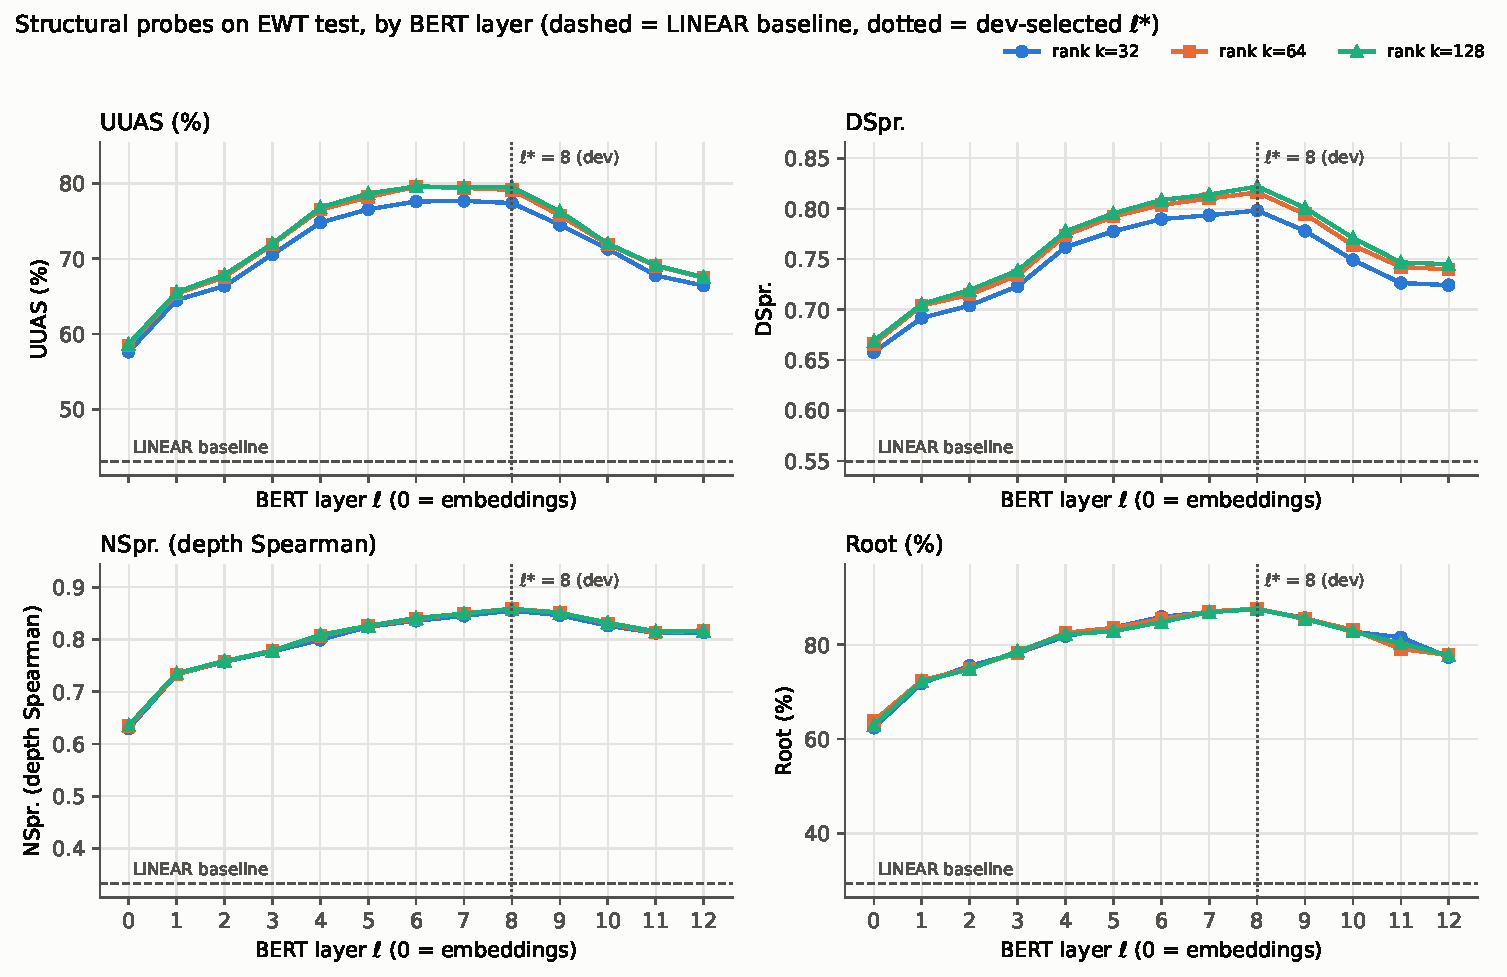
\includegraphics[width=0.93\textwidth]{metrics_vs_layer.pdf}
\caption{Probe metrics on EWT test vs.\ BERT layer, one line per rank (dashed = LINEAR baseline, dotted = dev-selected \lstar).}
\label{fig:layers}\end{figure}

\begin{table}[t]\centering\footnotesize\setlength{\tabcolsep}{4.2pt}\begin{tabular}{rccccccccc}
\toprule
 & \multicolumn{3}{c}{UUAS (\%), rank $k$} & & $\Delta$UUAS vs.\ $\ell^*$ (pt) & \multicolumn{3}{c}{NSpr (depth Spearman), $k$} & \\
\cmidrule(lr){2-4}\cmidrule(lr){7-9}
$\ell$ & 32 & 64 & 128 & DSpr & paired 95\% CI ($k{=}128$) & 32 & 64 & 128 & Root\% \\
\midrule
0 & 57.6 & 58.5 & 58.7 & 0.669 & $-$20.9 [$-$21.6, $-$20.1] & 0.629 & 0.634 & 0.636 & 63.0 \\
1 & 64.5 & 65.4 & 65.6 & 0.705 & $-$14.0 [$-$14.7, $-$13.2] & 0.733 & 0.733 & 0.735 & 72.2 \\
2 & 66.4 & 67.6 & 67.9 & 0.719 & $-$11.6 [$-$12.4, $-$10.9] & 0.757 & 0.758 & 0.759 & 74.8 \\
3 & 70.6 & 71.9 & 72.0 & 0.739 & $-$7.5 [$-$8.2, $-$6.8] & 0.777 & 0.779 & 0.778 & 78.3 \\
4 & 74.8 & 76.5 & 76.8 & 0.777 & $-$2.7 [$-$3.3, $-$2.1] & 0.799 & 0.807 & 0.809 & 82.2 \\
5 & 76.6 & 78.2 & 78.7 & 0.795 & $-$0.8 [$-$1.4, $-$0.3] & 0.824 & 0.827 & 0.826 & 82.9 \\
6 & 77.6 & 79.6 & 79.6 & 0.809 & +0.1 [$-$0.4, 0.6]$^\dagger$ & 0.836 & 0.839 & 0.841 & 84.8 \\
7 & 77.7 & 79.4 & 79.5 & 0.814 & 0.0 [$-$0.4, 0.5]$^\dagger$ & 0.845 & 0.850 & 0.850 & 87.0 \\
\rowcolor{black!8} 8 & 77.4 & 79.2 & 79.5 & 0.822 & -- & 0.855 & 0.859 & 0.859 & 87.5 \\
9 & 74.5 & 75.8 & 76.3 & 0.801 & $-$3.2 [$-$3.7, $-$2.8] & 0.846 & 0.852 & 0.851 & 85.5 \\
10 & 71.3 & 71.9 & 72.0 & 0.771 & $-$7.5 [$-$8.1, $-$7.0] & 0.826 & 0.831 & 0.832 & 82.8 \\
11 & 67.8 & 69.1 & 69.1 & 0.742 & $-$10.4 [$-$11.0, $-$9.8] & 0.812 & 0.813 & 0.815 & 80.3 \\
12 & 66.4 & 67.5 & 67.6 & 0.745 & $-$12.0 [$-$12.5, $-$11.4] & 0.814 & 0.818 & 0.816 & 77.8 \\
\midrule
LINEAR & \multicolumn{3}{c}{43.1} & 0.549 & -- & \multicolumn{3}{c}{0.333} & 29.4 \\
\bottomrule
\end{tabular}

\caption{Task 2 on EWT test, all layers and ranks. DSpr/Root\% use the dev-best rank of the layer. The $\Delta$ column is a
paired bootstrap of each layer vs.\ \lstar{} over the same sentences; $^\dagger$ = 95\% CI contains 0 (not significantly
different). Shaded: \lstar.}\label{tab:t2}\end{table}

\blk{Results (Fig.~\ref{fig:layers}, Table~\ref{tab:t2})}
\begin{itemize}
\item \textbf{Layer curve:} UUAS rises from \LzeroUUAS\% (layer 0) to a plateau over layers \TiedLayers{} and falls to \LtwelveUUAS\%
at layer 12; the depth probe has the same shape.
\item \textbf{Best layer:} dev selects \lstar=\Lstar{} (dev UUAS \TtwoDevUuas\%); depth also peaks at \Lstar{} on dev and test.
\item \textbf{Significance:} on test, layers \TiedLayers{} are statistically tied with \Lstar{} (the test argmax, layer \TtwoTestArgmax,
wins by 0.08\pt); every other layer is significantly worse.
\item \textbf{Rank:} at \lstar, UUAS \RankAUUAS{} / \RankBUUAS{} / \RankCUUAS\% and NSpr \RankANSpr{} / \RankBNSpr{} / \RankCNSpr{}
for $k=32/64/128$. The gain stops around $k=64$, as in the paper (Fig.~5): the tree lives in a $\approx$64-dimensional subspace.
\item \textbf{Convergence:} every probe reached its best dev loss by epoch 8--17.
\end{itemize}

\blk{What context adds}
\begin{itemize}
\item \textbf{Layer 0 is already strong:} word-piece + position embeddings with no context reach \LzeroUUAS\% -- far above LINEAR
(\LinUUAS\%) and close to the paper's non-contextual PROJ0 (59.8). Word identity plus position explains much of a tree.
\item \textbf{Context adds $\approx$21\pt,} the evidence that BERT's context encodes syntax.
\item \textbf{Biggest gains for function words,} which have no lexical cue to their head (recall, layer 0 $\to$ \Lstar): case
\PRelZeroCase$\to$\PRelCase, cc \PRelZeroCc$\to$\PRelCc, mark \PRelZeroMark$\to$\PRelMark, obl \PRelZeroObl$\to$\PRelObl.
\item \textbf{Smallest gains for adjacent pairs:} compound \PRelZeroCompound$\to$\PRelCompound, amod \PRelZeroAmod$\to$\PRelAmod.
\item \textbf{At \lstar:} easiest obj (\PRelObj), det (\PRelDet), aux (\PRelAux); hardest conj (\PRelConj) -- UD attaches every
conjunct to the first, creating long arcs -- and obl (\PRelObl), the PP-attachment ambiguity (heatmap in App.~\ref{app:figs}).
\end{itemize}

\needspace{9\baselineskip}\subsection{Comparison with the paper}\label{sec:paper}
\begin{table}[h]\centering\footnotesize\begin{tabular}{llcccc}
\toprule
 & system & UUAS & DSpr & Root\% & NSpr \\
\midrule
Paper (PTB WSJ) & LINEAR & 48.9 & 0.58 & 2.9 & 0.27 \\
Paper (PTB WSJ) & PROJ0 & 59.8 & 0.73 & 64.4 & 0.75 \\
Paper (PTB WSJ) & ELMO1 & 77.0 & 0.83 & 86.5 & 0.87 \\
Paper (PTB WSJ) & BERTBASE7 & 79.8 & 0.85 & 88.0 & 0.87 \\
Paper (PTB WSJ) & BERTLARGE16 & 81.7 & 0.87 & 90.1 & 0.89 \\
\midrule
Ours (EWT) & LINEAR (word order only) & 43.1 & 0.549 & 29.4 & 0.333 \\
Ours (EWT) & BERT layer 0 (embeddings + position) & 58.7 & 0.669 & 63.0 & 0.636 \\
Ours (EWT) & \textbf{BERT-base-uncased layer 8} (paper schedule) & 79.5 & 0.822 & 87.5 & 0.859 \\
Ours (EWT) & BERT layer 8, spec-literal (constant lr, last epoch) & 62.0 & 0.760 & 58.6 & 0.803 \\
\bottomrule
\end{tabular}

\caption{Our numbers vs.\ \citet{hewitt} Table~1 (PTB WSJ test, BERT-base \emph{cased}, Stanford Dependencies).}
\label{tab:paper}\end{table}
\begin{itemize}
\item \textbf{The result reproduces:} within 0.3\pt{} UUAS, 0.03 DSpr, 0.5\pt{} Root\% and 0.01 NSpr of the paper's BERTBASE7.
\item \textbf{Non-contextual baseline:} our layer-0 probe matches their PROJ0 (UUAS 58.7 vs.\ 59.8).
\item \textbf{Layer numbering:} the paper counts BERT-base layers 0--11 without the embedding layer, so its ``layer 7'' is our HF
layer 8 (or 7 under the other reading); layers \TiedLayers{} are tied, so the comparison holds either way.
\item \textbf{Likely causes of the small DSpr/NSpr gap} (plausible, not isolated):
\begin{enumerate}
\item \textbf{data scale} -- 12.5k train sentences vs.\ $\approx$40k in PTB;
\item \textbf{genre} -- web text with typos and fragments vs.\ edited news;
\item \textbf{annotation} -- UD's content-head trees (prepositions and copulas are dependents) vs.\ Stanford Dependencies;
\item \textbf{casing} -- uncased vs.\ cased model;
\item \textbf{budget} -- rank $\le$128 and 30 epochs vs.\ full rank and up to 40 epochs.
\end{enumerate}
\item \textbf{LINEAR differs more} (UUAS \LinUUAS{} vs.\ 48.9; Root\% \LinRoot{} vs.\ 2.9): EWT sentences are short and often
\emph{start with their root} (``Say \ldots'', ``Thanks \ldots'', fragments), whereas WSJ sentences start with a subject.
\end{itemize}

\needspace{9\baselineskip}\subsection{Control run: the assignment's literal training schedule}\label{sec:literal}
\begin{itemize}
\item \textbf{Why:} the assignment specifies Adam with lr $10^{-3}$ for 30 epochs; we added the paper's lr decay and best-dev selection.
\item \textbf{Run:} every layer retrained ($k=128$) with constant lr $10^{-3}$, keeping the epoch-30 probe.
\item \textbf{Same conclusion:} \lstar{} is unchanged (\LitLstar{} on dev and test) and the curve keeps its rise--peak--fall shape.
\item \textbf{Much lower level:} UUAS at \lstar{} drops to \LitUuas\% (DSpr \LitDspr, NSpr \LitNspr, Root \LitRoot\%; Table~\ref{tab:paper}).
\item \textbf{Cause -- non-convergence:} at layer 8 the \emph{training} loss stays at 0.62 (vs.\ 0.42 with decay) and the dev loss oscillates
between 0.54 and 0.59 for 30 epochs. With an L1 loss the gradient does not shrink near the optimum, so Adam's steps stay $\approx$lr and
circle the minimum; the decay lets the probe converge.
\item \textbf{Verdict:} the deviation is necessary for a faithful reproduction, and the main conclusion (\lstar=8) does not depend on it.
\end{itemize}

% =====================================================================================================
\needspace{11\baselineskip}\section{Task 3 -- BERT-derived static vectors}\label{sec:t3}
\blk{Method}
\begin{itemize}
\item \textbf{Pooling:} for each of the \VocabTypes{} T1 word types, average its layer-\lstar{} vectors (each the mean of its word pieces,
computed \emph{in context}) over all its occurrences in EWT train -- the mean/mean pooling that \citet{bommasani} found best.
\item \textbf{Identical protocol:} same vocabulary and row order as T1; WS-353, analogy and the 20-sentence MST run through \emph{the same
function} as T1.
\end{itemize}
\blk{Additions beyond the spec}
\begin{enumerate}[label=(\alph*)]
\item \textbf{All-but-the-top} \citep{mu}: subtract the mean and remove the top $D=d/100$ principal directions ($D=7$ for BERT), because
pooled BERT vectors are anisotropic \citep{ethayarajh}; also applied to T1 ($D=1$) so post-processing is not credited to BERT.
\item \textbf{Paired significance tests} on identical items: bootstrap of $\Delta\rho$ over pairs, exact McNemar over analogy
questions, bootstrap of $\Delta$UUAS over sentences.
\item \textbf{Layer sweep} over layers 0--12.
\item \textbf{Diagnostic ladder} of MSTs on the same sentences.
\item \textbf{Combination variants:} concatenated L2-normalised [T1;\,T3] vectors, and T3 vectors seen through the T2 probe matrix $B$.
\end{enumerate}

\begin{table}[t]\centering\footnotesize\setlength{\tabcolsep}{3.6pt}\resizebox{\textwidth}{!}{\begin{tabular}{lccccccc}
\toprule
 & \multicolumn{2}{c}{WordSim-353 $\rho$} & \multicolumn{3}{c}{Analogy acc.\ (\%)} & \multicolumn{2}{c}{MST UUAS (\%)} \\
\cmidrule(lr){2-3}\cmidrule(lr){4-6}\cmidrule(lr){7-8}
system & covered [95\% CI] & all 353 & covered & sem / syn & all & 20 sent.\ [95\% CI] & pool \\
\midrule
T1 PPMI-SVD (spec) & 0.104 [$-$0.03, 0.22] & 0.048 & 0.5 & 2.1 / 0.3 & 0.1 & 20.5 [16.3, 26.2] & 24.8 \\
T1 PPMI-SVD, best variant ($p{=}0$) & 0.134 [0.00, 0.25] & 0.089 & 0.2 & 0.9 / 0.1 & 0.1 & 22.6 [17.8, 28.4] & 24.5 \\
\textbf{T3 BERT-static, layer 8} & 0.577 [0.47, 0.66] & 0.452 & 67.7 & 74.5 / 66.6 & 19.8 & 18.4 [13.6, 26.0] & 17.9 \\
T3 + all-but-the-top ($D{=}7$) & 0.682 [0.61, 0.74] & 0.539 & 71.0 & 79.0 / 69.7 & 20.8 & 19.7 [14.9, 26.2] & 19.6 \\
\midrule
T2 probe, layer 8 (contextual, supervised; reference) & -- & -- & -- & -- & -- & 81.2 [75.9, 85.9] & 82.9 \\
linear chain / random tree & -- & -- & -- & -- & -- & 43.2 / 15.2 & 43.0 / 17.1 \\
\bottomrule
\end{tabular}
}
\caption{Task 3 vs.\ Task 1 (identical items), with the Task 2 probe as a reference on the same 20 sentences and pool.}
\label{tab:t3}\end{table}
\begin{table}[t]\centering\footnotesize\setlength{\tabcolsep}{4pt}\begin{tabular}{lccccc}
\toprule
 & WordSim-353 & \multicolumn{2}{c}{Analogy (McNemar)} & \multicolumn{2}{c}{MST $\Delta$UUAS (pt) [95\% CI]} \\
\cmidrule(lr){3-4}\cmidrule(lr){5-6}
A $-$ B & $\Delta\rho$ [95\% CI] & only A / only B & $p$ & 20 sentences & pool (660) \\
\midrule
T3 $-$ T1 & +0.474 [0.36, 0.61] & 3,848 / 0 & $<10^{-300}$ & $-$2.1 [$-$6.4, 3.2] & $-$6.9 [$-$8.0, $-$5.8] \\
T3+ABTT $-$ T1 & +0.579 [0.46, 0.71] & 4,036 / 0 & $<10^{-300}$ & $-$0.9 [$-$6.6, 5.6] & $-$5.1 [$-$6.2, $-$4.1] \\
T3+ABTT $-$ T3 & +0.105 [0.05, 0.16] & 276 / 88 & $1\times10^{-23}$ & +1.3 [$-$3.2, 5.6] & +1.7 [1.0, 2.6] \\
T2 probe $-$ T3 & -- & -- & -- & +62.8 [53.2, 69.6] & +65.0 [63.8, 66.3] \\
\bottomrule
\end{tabular}

\caption{Paired tests on identical items. Analogy: number of questions solved by only A / only B, exact McNemar $p$.}
\label{tab:tests}\end{table}

\blk{Word meaning: T3 is much better (Tables~\ref{tab:t3}, \ref{tab:tests})}
\begin{itemize}
\item \textbf{WS-353:} \TOneWSCov{} $\to$ \TThreeWSCov{} on covered pairs ($\Delta\rho=\PtWSDiff$, CI \PtWSCI) and \TOneWSFull{} $\to$
\TThreeWSFull{} on all 353; all-but-the-top adds another \PtAbttWSDiff{} (\TThreeAWSCov).
\item \textbf{Analogies:} \TOneANCov\% $\to$ \TThreeANCov\% on covered questions (\TThreeAANCov\% with ABTT) and \TThreeANFull\% on all
\ANTotal; T3 solves \PtANOnlyA{} questions T1 misses, T1 solves \PtANOnlyB{} that T3 misses.
\item \textbf{Rare words too:} $\rho=\TThreeWSCov$ on all covered pairs vs.\ \TThreeWSFreqTwenty{} on frequent ones -- BERT's knowledge comes
from pre-training ($\approx$3.3B words), not from EWT, so this win is expected.
\item \textbf{Agrees with the literature:} our best WS-353 layer is layer~\BestSemLayer{} ($\rho=\BestSemWS$, $\approx$6.8k contexts);
\citet{bommasani} report 0.683 at layer~1 for bert-base-uncased with 10k contexts.
\end{itemize}

\blk{Tree structure: T3 is worse}
\begin{itemize}
\item \textbf{20 required sentences:} T3 \TThreeMST\% vs.\ T1 \TOneMST\% ($\Delta=\PtMSTDiff$\pt, CI \PtMSTCI) -- \emph{not significant};
20 sentences cannot separate them.
\item \textbf{660-sentence pool:} T3 \TThreePool\% vs.\ T1 \TOnePool\% ($\Delta=\PtPoolDiff$\pt, CI \PtPoolCI) -- significant, and
barely above a random tree (\RandomPool\%).
\item \textbf{Reference:} the T2 probe reaches \TTwoRefMST\% / \TTwoRefPool\% on the same sentences.
\item \textbf{So the two evaluations disagree:} pooling from the syntax layer gives much better vectors by the standard benchmarks and
worse ones by the structural check.
\end{itemize}

\begin{figure}[t]\centering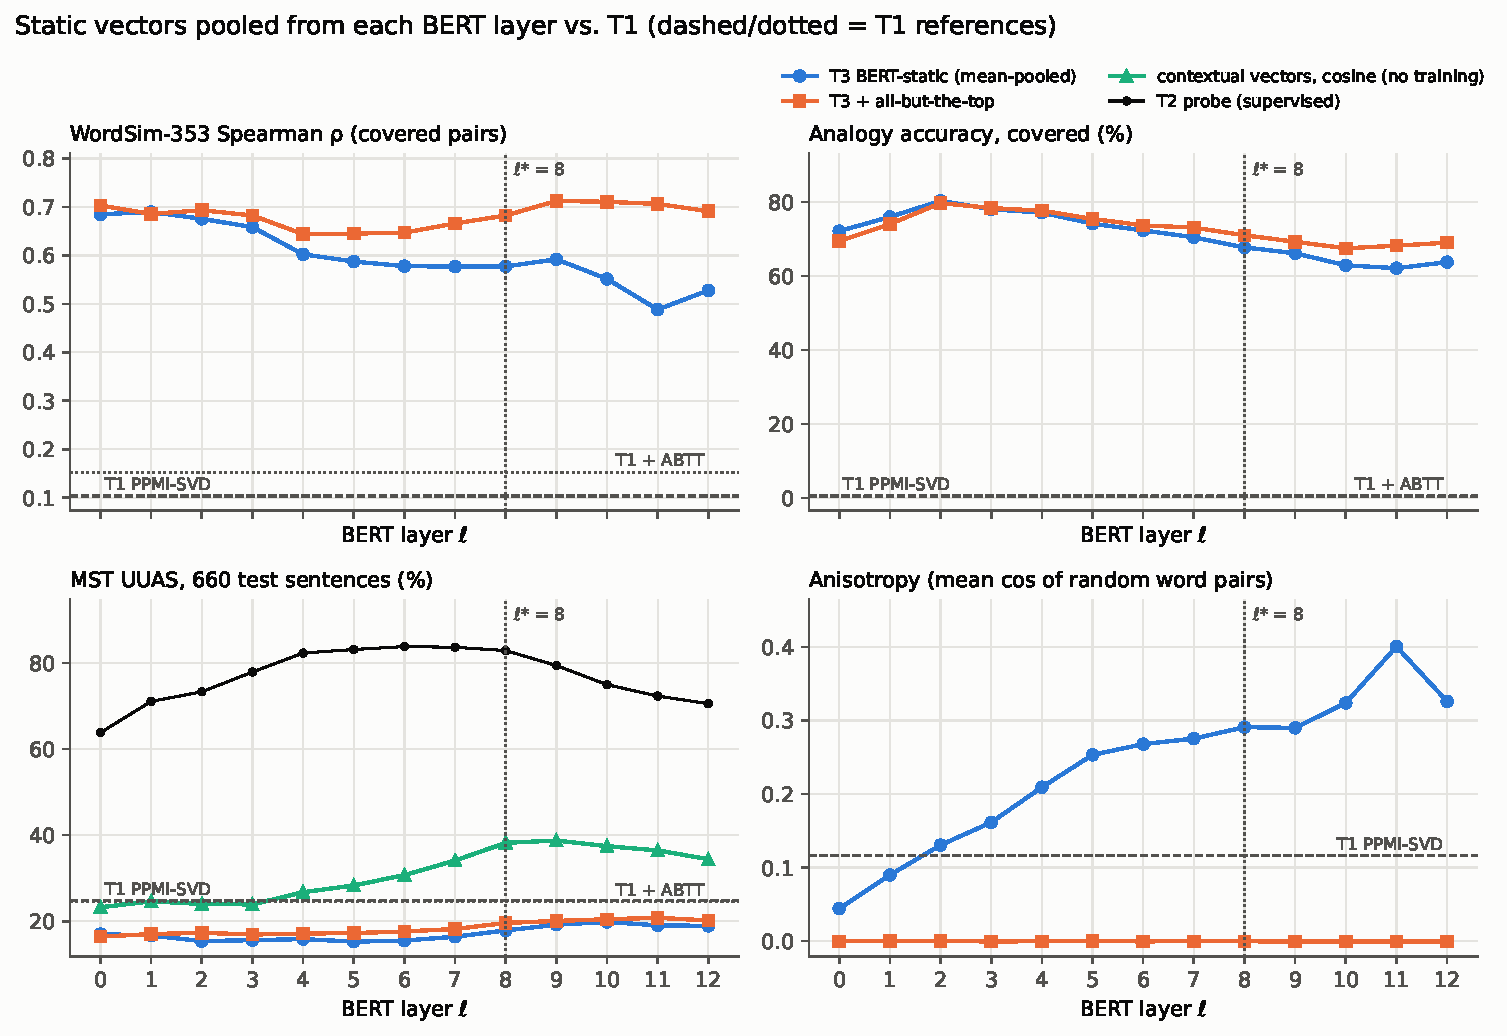
\includegraphics[width=0.93\textwidth]{layer_sweep.pdf}
\caption{Static vectors pooled from every BERT layer (raw and with all-but-the-top) vs.\ T1 references; the MST panel also
shows raw contextual vectors (cosine, no training) and the T2 probe on the same 660 sentences. Numbers in App.~\ref{app:tabs}.}
\label{fig:sweep}\end{figure}

\blk{Is the syntax layer the right layer for static semantics? No (Fig.~\ref{fig:sweep})}
\begin{itemize}
\item \textbf{Best static layers are the lowest:} WS-353 peaks at layer~\BestSemLayer{} (\BestSemWS), analogies at layer~\BestAnLayer{}
(\BestAnAcc\%); even layer~0 (essentially the input embedding table) gives $\rho=\LzeroWS$ and \LzeroAn\%. This matches \citet{bommasani}.
\item \textbf{Anisotropy explains the decline:} raw WS falls with depth while the mean cosine of random word pairs rises from \AnisoLzero{} to
\AnisoMax{} (layer \AnisoMaxLayer); after all-but-the-top the WS curve is almost flat (\AbttWSMin--\AbttWSMax).
\item \textbf{Analogies still decline after ABTT:} upper layers are more context-specific.
\item \textbf{No layer helps trees:} static MST UUAS is \StaticMSTMin--\StaticMSTMax\% at every layer.
\end{itemize}

\needspace{9\baselineskip}\subsection{Why the evaluations disagree -- measured, not assumed}\label{sec:why}
\begin{table}[t]\centering\footnotesize\setlength{\tabcolsep}{4pt}\begin{tabular}{llccc}
\toprule
representation for the MST & tier & 20 sentences [95\% CI] & pool (660) [95\% CI] & edge AUC \\
\midrule
random tree (expected) & -- & 15.2 & -- & -- \\
linear chain & -- & 43.2 [40.6, 46.4] & 43.0 [42.4, 43.7] & 0.75 \\
T1 PPMI-SVD (spec) & req. & 20.5 [16.3, 26.2] & 24.8 [23.7, 26.0] & 0.54 \\
T1 PPMI-SVD (p0) & B & 22.6 [17.8, 28.4] & 24.5 [23.4, 25.6] & -- \\
T3 BERT-static L8 & req. & 18.4 [13.6, 26.0] & 17.9 [16.8, 18.9] & 0.46 \\
T3 BERT-static L8 + ABTT & B & 19.7 [14.9, 26.2] & 19.6 [18.6, 20.7] & 0.44 \\
concat [T1 ; T3] (L2-normalised) & C & 19.2 [15.2, 25.1] & 25.1 [24.0, 26.2] & -- \\
T3 BERT-static L8 through probe B & C & 29.5 [23.7, 38.2] & 35.9 [34.3, 37.5] & -- \\
contextual L8, cosine (no training) & B & 35.9 [32.1, 39.6] & 38.2 [37.3, 39.2] & 0.70 \\
T2 distance probe L8 k=128 & ref. & 81.2 [75.9, 85.9] & 82.9 [81.9, 83.9] & 0.96 \\
\bottomrule
\end{tabular}

\caption{The diagnostic ladder on the same sentences. Edge AUC: within each pool sentence, the probability that a gold edge
pair is closer than a non-edge pair (0.5 = no information), averaged over sentences. Tier: req.\ = required, B/C = our extensions.}
\label{tab:ladder}\end{table}
\begin{table}[t]\centering\footnotesize\setlength{\tabcolsep}{4pt}\begin{tabular}{lcccc}
\toprule
 & T1 PPMI-SVD & T3 layer 8 & T3 + ABTT & random / gold \\
\midrule
NN with same majority UPOS (top-10) & 0.326 & 0.740 & 0.710 & 0.223 \\
NN that co-occur within $\pm5$ in train & 0.557 & 0.162 & 0.156 & 0.067 \\
hubness: skewness of $N_{10}$ & 2.10 & 1.45 & 0.57 & -- \\
function words among top-50 hubs & 0.10 & 0.12 & 0.02 & -- \\
\midrule
edge AUC (gold edge closer than non-edge) & 0.54 & 0.46 & 0.44 & 0.50 \\
MST: mean degree of function-word tokens & 1.84 & 2.29 & 2.04 & 1.05 (gold) \\
MST: mean max.\ degree per sentence & 3.75 & 5.46 & 3.62 & 4.53 (gold) \\
MST: edges joining same-UPOS words & 0.21 & 0.25 & 0.29 & 0.13 (gold) \\
\bottomrule
\end{tabular}

\caption{Diagnostics (\texttt{diagnostics\_task3.py}). NN statistics use the 2,134 types with train frequency $\ge$10 and the
majority UPOS of each type; hubness uses the 3,919 types with frequency $\ge$5; MST statistics use the 660-sentence pool.}
\label{tab:diag}\end{table}

\begin{enumerate}
\item \textbf{The tree lives in the context, and pooling averages it away} (Table~\ref{tab:ladder}).
\begin{itemize}
\item The ladder adds one ingredient per rung: static T3 \TThreePool\% $\to$ the same vectors through the probe's subspace $B$
\LadProjPool\% $\to$ per-token contextual vectors, plain cosine \LadCtxPool\% $\to$ the trained probe \TTwoRefPool\%.
\item Averaging ``bank'' over all its sentences gives a good dictionary entry, but cannot know what ``bank'' attaches to in
\emph{this} sentence.
\item Even raw contextual vectors stay below the linear chain (\ChainPool\%): BERT's tree is in a learned low-rank subspace, not in its raw
cosine geometry -- exactly the structural probe's claim.
\end{itemize}
\item \textbf{``Similar'' is not ``connected'' (paradigmatic vs.\ syntagmatic, \citealt{sahlgren}).}
\begin{itemize}
\item \textbf{T3 finds substitutes:} \NNSameTThree{} of its 10 nearest neighbours share the word's part of speech (T1 \NNSameTOne; random
\NNSameRandom), e.g.\ good $\to$ excellent, great (Table~\ref{tab:nn}).
\item \textbf{T1 finds partners:} \NNCoocTOne{} of its neighbours co-occur with the word within $\pm$5 (T3 \NNCoocTThree; random
\NNCoocRandom), e.g.\ said $\to$ spokesman, car $\to$ driving.
\item \textbf{Direct test, edge AUC:} inside a sentence, T3 closeness carries \emph{no} information about attachment (\AucTThree, slightly
below chance); T1 a little (\AucTOne); contextual vectors (\AucCtx), word order (\AucChain) and the probe (\AucProbe) are informative.
\item \textbf{Per relation:} T1 beats T3 on head--dependent pairs -- nsubj (\TOneRelNsubj{} vs.\ \TThreeRelNsubj), obj (\TOneRelObj{} vs.\
\TThreeRelObj), amod (\TOneRelAmod{} vs.\ \TThreeRelAmod); T3 wins only on conj (\TThreeRelConj{} vs.\ \TOneRelConj), the relation that
links two \emph{similar} words (``cats and dogs'').
\item \textbf{A first guess, corrected:} ``gold edges join different categories'' is \emph{not} supported -- gold edges are same-UPOS
slightly \emph{more} often than non-edges (\GoldSameUpos{} vs.\ \GoldSameUposNon); the AUC result is what matters.
\end{itemize}
\item \textbf{Within-sentence hubs.}
\begin{itemize}
\item Over the whole vocabulary T3 is \emph{not} more hub-prone than T1 (skewness of the 10-NN in-degree $N_{10}$ \citep{radovanovic}:
\SkewTThree{} vs.\ \SkewTOne).
\item Inside sentences T3's MSTs are star-shaped around frequent function words: function-word tokens get \FnDegTThree{} edges on
average (gold \FnDegGold, T1 \FnDegTOne); the largest degree per sentence is \MaxDegTThree{} (gold \MaxDegGold).
\item All-but-the-top reduces both (Table~\ref{tab:diag}) and gives the significant +1.7\pt{} on the pool, but does not fix the tree.
\end{itemize}
\end{enumerate}

\blk{Combination variants}
\begin{itemize}
\item \textbf{Concatenation [T1;\,T3]} hurts semantics (WS \ConcatWS, analogy \ConcatAN\% -- T1's noisy similarities dilute BERT's) and only
matches T1 on trees (\LadConcatPool\%): the two spaces are not usefully complementary.
\item \textbf{T3 through the probe's $B$} doubles its tree score (\LadProjPool\%): the syntactic subspace carries some \emph{type-level}
information (which kind of word attaches to which), but most of the tree requires context.
\end{itemize}

% =====================================================================================================
\needspace{11\baselineskip}\section{Qualitative analysis}\label{sec:qual}
\blk{Task 2: probe errors (examples chosen by rank among test sentences with 10--18 words, not by hand)}
\begin{itemize}
\item \textbf{Best} (UUAS \QGoodUUAS): ``\QGoodText'' -- every edge correct.
\item \textbf{Median} (\QTypicalUUAS): ``\QTypicalText''.
\begin{itemize}
\item missed: \QTypicalMissed; spurious: \QTypicalSpurious;
\item the probe joins the two subjects ``I'' to each other instead of linking the clauses through their verbs, and misreads the
discourse use of ``Say''.
\end{itemize}
\item \textbf{Worst} (\QPoorUUAS): the verbless itinerary ``\QPoorText''.
\begin{itemize}
\item the probe links \emph{repeated identical words} (to--to, Chicago--Chicago) and chains the cities left to right, whereas UD
attaches each conjunct to the first;
\item identical word forms get very similar BERT vectors, so lexical identity leaks into the syntactic distance -- the most frequent
failure we saw, together with coordination and PP attachment.
\end{itemize}
\end{itemize}
\begin{figure}[t]\centering
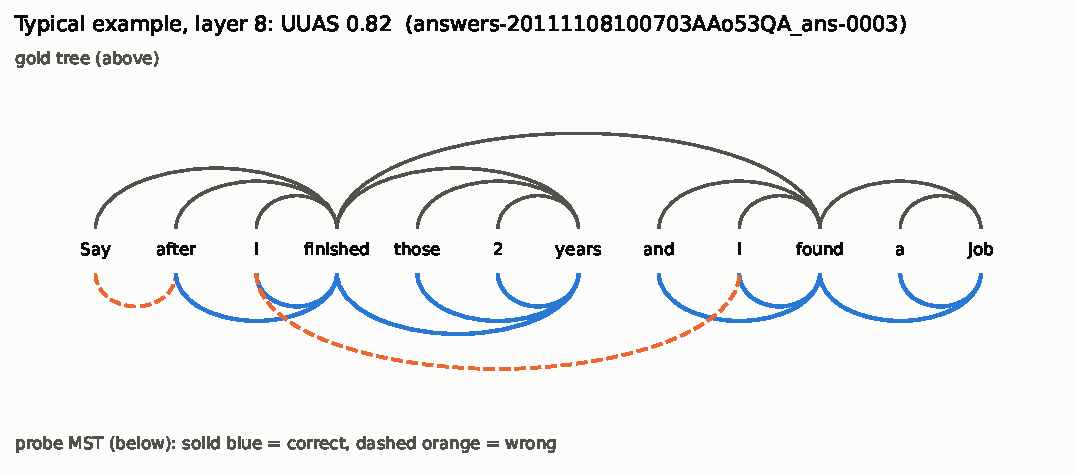
\includegraphics[width=0.78\textwidth]{example_typical.pdf}\\[2pt]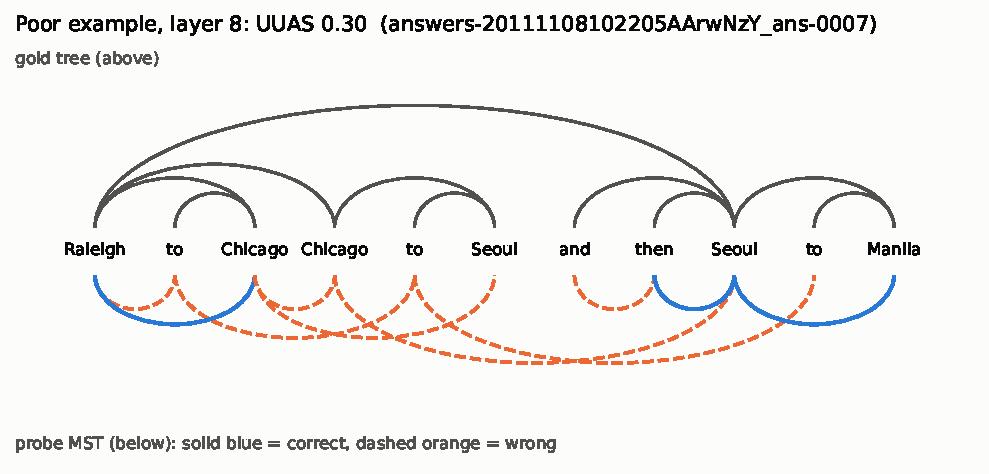
\includegraphics[width=0.78\textwidth]{example_poor.pdf}
\caption{T2 probe (layer \Lstar) on the median (top) and the worst (bottom) test sentence of 10--18 words. Gold tree above the words, probe MST below:
blue solid = correct, orange dashed = wrong.}\label{fig:t2ex}\end{figure}

\begin{table}[t]\centering\footnotesize\setlength{\tabcolsep}{4pt}\begin{tabular}{lll}
\toprule
word & T1 PPMI-SVD: 5 nearest neighbours & T3 BERT-static (layer 8): 5 nearest neighbours \\
\midrule
\textit{good} & nice, food, pretty, great, really & excellent, great, nice, decent, wonderful \\
\textit{bad} & faith, big, too, wrong, something & terrible, horrible, poor, good, shitty \\
\textit{monday} & friday, 0832, july, sunday, 6 & tuesday, sunday, thursday, wednesday, saturday \\
\textit{dog} & got, horse, cat, myself, leave & dogs, cat, puppy, animal, cats \\
\textit{car} & home, guy, test, driving, drive & cars, vehicle, vehicles, suv, ferrari \\
\textit{money} & save, enough, much, else, attention & cash, funds, dollars, cashout, bucks \\
\textit{said} & spokesman, nun, penman, gregg, maviglio & says, stated, saying, told, say \\
\textit{happy} & definitely, customer, guys, !!, safe & pleased, glad, unhappy, satisfied, delighted \\
\textit{computer} & disc, plans, evidence, read, mohammed & laptop, computers, pc, machine, internet \\
\textit{two} & screamed, paddled, expressway, kitchens, revolt & three, four, 2, five, six \\
\bottomrule
\end{tabular}

\caption{Nearest neighbours (cosine). T1 finds co-occurring partners (and noise from rare words); T3 finds substitutes.}
\label{tab:nn}\end{table}
\begin{table}[t]\centering\footnotesize\setlength{\tabcolsep}{4pt}\begin{tabular}{llll}
\toprule
section & question ($a:b::c:$\,\textbf{gold}) & T3 answer & T1 answer \\
\midrule
capital-common-countries & baghdad : iraq :: beijing : \textbf{china} & china \checkmark & jintao \\
capital-world & amman : jordan :: baghdad : \textbf{iraq} & iraq \checkmark & threats \\
city-in-state & houston : texas :: philadelphia : \textbf{pennsylvania} & pennsylvania \checkmark & franchise \\
family & boy : girl :: brother : \textbf{sister} & sister \checkmark & cousin \\
gram1-adjective-to-adverb & amazing : amazingly :: complete : \textbf{completely} & completely \checkmark & digest \\
gram2-opposite & acceptable : unacceptable :: aware : \textbf{unaware} & unaware \checkmark & socially \\
\midrule
capital-world & beijing : china :: kingston : \textbf{jamaica} & jamaican & northwest \\
currency & brazil : real :: canada : \textbf{dollar} & actual & church \\
gram2-opposite & acceptable : unacceptable :: certain : \textbf{uncertain} & specific & socially \\
gram3-comparative & bad : worse :: cool : \textbf{cooler} & nicer & dried \\
gram4-superlative & bad : worst :: big : \textbf{biggest} & largest & chinese \\
gram6-nationality-adjective & australia : australian :: england : \textbf{english} & british & soper \\
\bottomrule
\end{tabular}

\caption{Analogy examples: top, questions T3 solves and T1 does not (one per section); bottom, T3 failures.}
\label{tab:analogy}\end{table}

\blk{Task 3: neighbours, analogies and one sentence}
\begin{itemize}
\item \textbf{Neighbours} (Table~\ref{tab:nn}) show the paradigmatic/syntagmatic contrast directly; T1's lists for mid-frequency words
(\emph{two}, \emph{computer}) are noise from rare co-occurrences.
\item \textbf{Analogy successes} (Table~\ref{tab:analogy}): near-perfect on regular morphology (plural \TThreePlural\%) and frequent
capitals (\TThreeCapital\%).
\item \textbf{Analogy failures:} ambiguous or rare answers -- currency (\TThreeCurrency; ``real'' occurs 53 times in EWT train, always as an
adjective) and opposites (\TThreeOpposite\%).
\item \textbf{Near misses:} T3 picks a semantic neighbour over the morphological target (cooler $\to$ nicer, biggest $\to$ largest,
english $\to$ british) -- the substitute bias again. T1's wrong answers are unrelated co-occurring words (Baghdad:Iraq::Beijing $\to$ \emph{jintao}).
\item \textbf{A representative sentence} (Fig.~\ref{fig:mstex}; chosen as the one whose per-method scores are closest to each method's
average): T1 and T3 each get \ExTOne\%, raw contextual vectors \ExCtx\%, the probe \ExProbe\%; the T3 tree is a star around ``a'' and ``of''.
\end{itemize}
\begin{figure}[t]\centering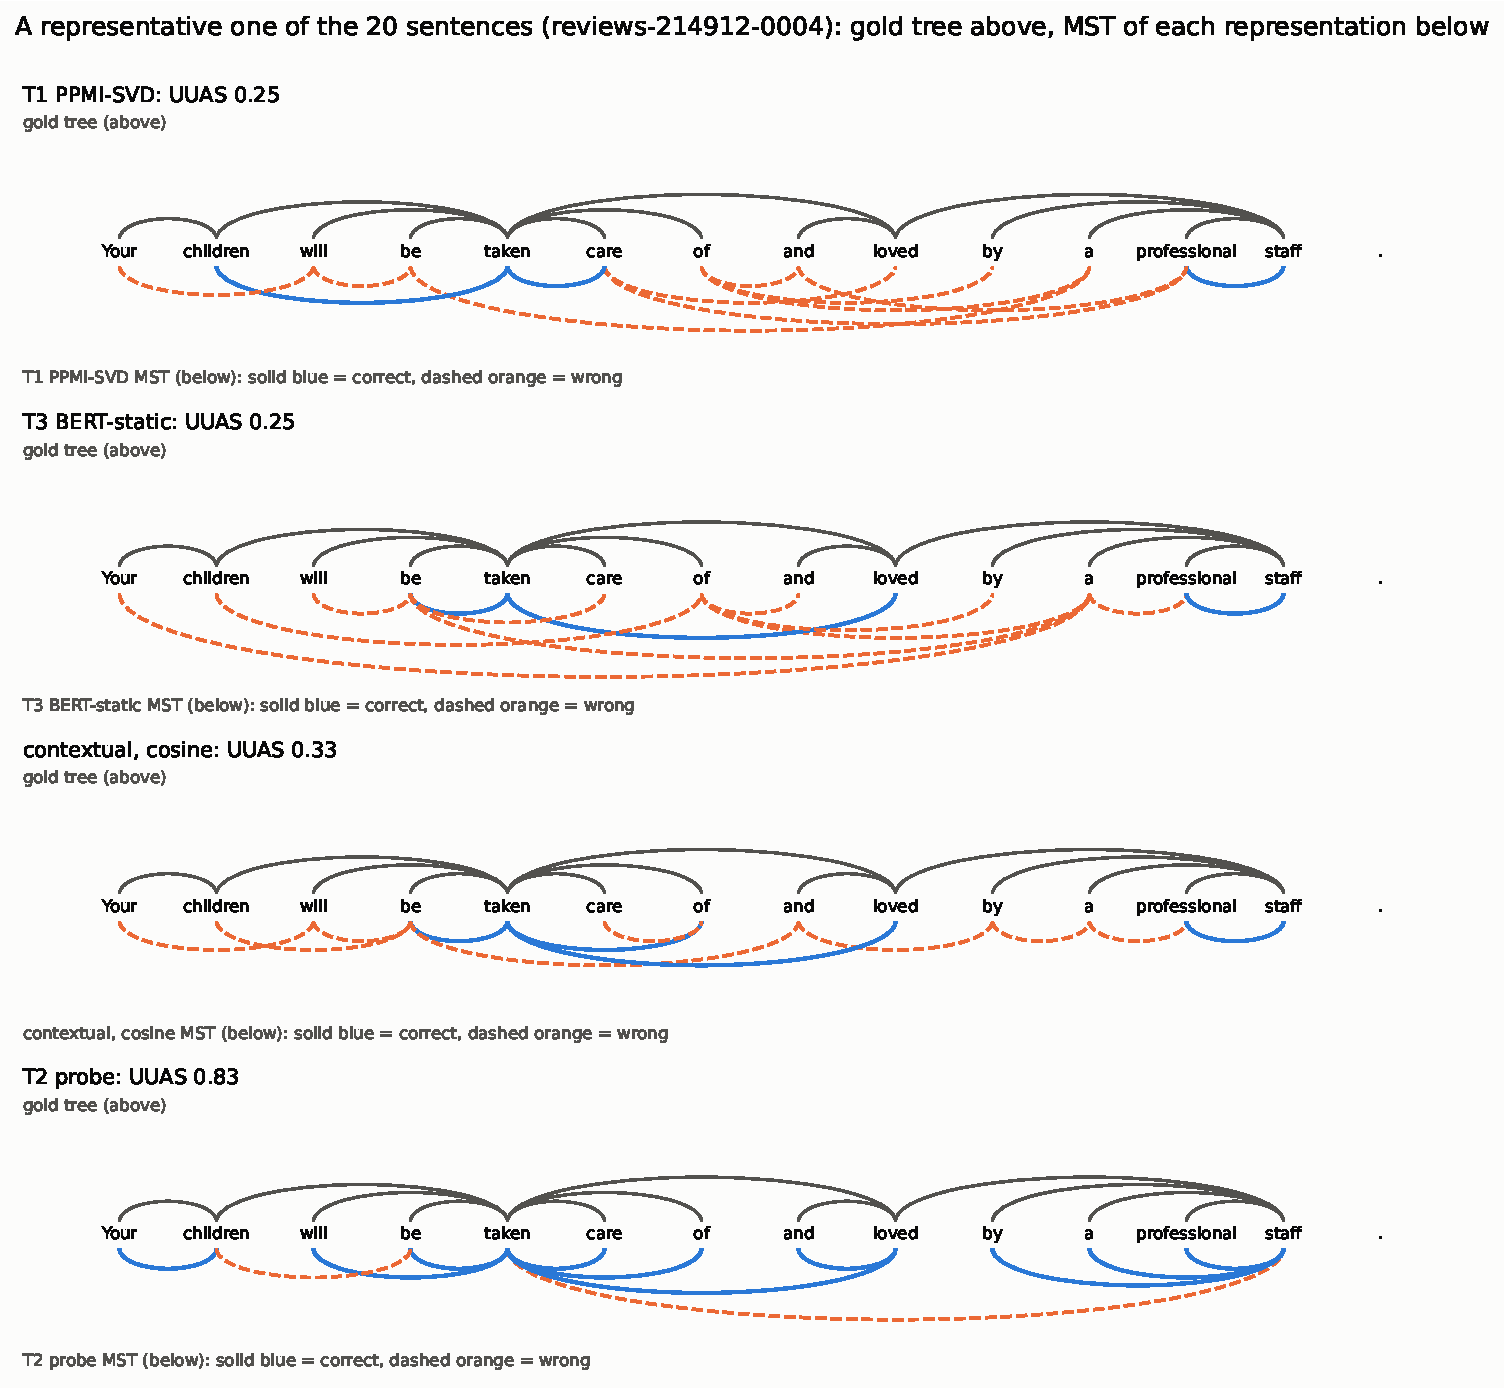
\includegraphics[width=0.80\textwidth]{mst_example.pdf}
\caption{``\ExText'' -- gold tree (above) and the MST of each representation (below).}\label{fig:mstex}\end{figure}

% =====================================================================================================
\needspace{11\baselineskip}\section{Discussion}\label{sec:disc}
\blk{What worked}
\begin{itemize}
\item The structural probe reproduces on a different treebank, genre and annotation scheme: same peak layers, same rank saturation,
within 0.3\pt{} UUAS.
\item Pooled BERT vectors are strong lexical-semantic vectors even from 200k words of text, because the knowledge was learned in pre-training.
\item One cheap post-processing step (all-but-the-top) adds a significant $+$0.1 $\rho$.
\item Paired tests, the 660-sentence pool and bootstrap CIs separated real effects from noise (the 6--8 layer plateau; the
non-significant 20-sentence T1/T3 difference).
\end{itemize}
\blk{What did not work, and why}
\begin{enumerate}
\item \textbf{PPMI-SVD on 200k words} cannot do analogies and only weakly captures similarity -- data sparsity, confirmed by the
frequency analysis and by the failure of every Levy et al.\ variant.
\item \textbf{Pooling the syntax layer does not give syntactic vectors.} The structural check rewards \emph{syntagmatic} association
between words of one sentence; averaging removes the token-specific information that makes BERT syntactic, leaving substitute-style
similarity that is uninformative about attachment (edge AUC \AucTThree).
\item \textbf{The layer is mismatched:} the syntax layer (\Lstar) is not the best static-semantics layer (\BestSemLayer--\BestAnLayer).
\item \textbf{The spec's constant learning rate} does not let an L1-loss probe converge.
\end{enumerate}
\blk{Do the two answers agree? No}
\begin{itemize}
\item Semantic benchmarks measure paradigmatic similarity between word \emph{types}; the tree check measures syntagmatic relations
between \emph{tokens}.
\item A representation can -- and here does -- improve on one while getting worse on the other.
\end{itemize}
\blk{Limitations}
\begin{itemize}
\item One treebank and one model.
\item The 20-sentence check is under-powered (hence the pool), and the sample is biased towards in-vocabulary, 5--40-word sentences.
\item BERT brings 3.3B words of external knowledge, so T1 vs.\ T3 is not a same-data comparison.
\item The causes of the DSpr/NSpr gap are plausible but not isolated.
\end{itemize}

% =====================================================================================================
\needspace{11\baselineskip}\section{Reproducibility, seeds and deviations}\label{sec:repro}
\begin{itemize}
\item \textbf{Seeds:} \texttt{SEED = 42} (\texttt{code/common/config.py}) seeds Python, NumPy and PyTorch (\texttt{PYTHONHASHSEED} set).
It drives the 20-sentence sample (\texttt{numpy.random.default\_rng(42)}), the random-tree baseline, all bootstraps (1000 resamples), the SVD
(\texttt{random\_state=42}) and the anisotropy sampling. Probe $(\ell,k,\text{type})$ is initialised with seed $42+1000\ell+k$ (+500 for
depth); batch order uses seed $42+\ell$.
\item \textbf{Environment:} Python 3.12, PyTorch 2.15, Transformers 5.22, Datasets 5.1 (pinned in \texttt{requirements.txt}); 2$\times$NVIDIA L40S (shared).
\item \textbf{Runtime:} T1 seconds; BERT features 7\,min; 78 probes 49+54\,min on two GPUs; T3 $<$5\,min.
\item \textbf{Pretrained checkpoint:} \texttt{google-bert/bert-base-uncased}, Hugging Face Hub, revision \texttt{86b5e09}.
\item \textbf{Code:} \texttt{code/task1}, \texttt{task2}, \texttt{task3} (plus \texttt{common/} for data loading and the shared evaluation);
\texttt{run\_all.py} and a Colab notebook run everything end-to-end (README).
\end{itemize}

\begin{table}[H]\centering\footnotesize\setlength{\tabcolsep}{4pt}
\begin{tabular}{p{0.27\textwidth}p{0.68\textwidth}}
\toprule
Deviation / interpretation & Justification \\
\midrule
Window ``size 5'' = 5 words each side & Standard reading \citep{levy2015}; counts never cross sentence boundaries. \\
Lowercasing (T1, T3, benchmarks) & The model is uncased; T1 and T3 then share one vocabulary, so their coverage is identical. \\
WS-353 reported on all 353 pairs \emph{and} on the 248 covered & ``All 353'' is the spec-literal number (OOV pairs get the median similarity, a neutral rank; a 0 would be non-neutral for anisotropic BERT); ``covered'' is the informative comparison. Analogy: OOV questions count wrong in ``all''. \\
20-sentence sample: 5--40 words, all in vocabulary; punctuation ignored & A static model has no vector for an OOV word; punctuation is excluded exactly as in the probe paper. The bias towards simpler sentences is acknowledged. \\
LR $\times$0.1 on dev plateau + best-dev checkpoint (T2) & The paper's schedule; the spec-literal control (\S\ref{sec:literal}) keeps \lstar{} but does not converge. \\
Layer 0 probed in addition to 1--12 & Non-contextual baseline (cf.\ the paper's PROJ0). \\
\lstar{} chosen on dev, not test & Avoids test-set selection; the 6--8 plateau makes the choice robust. \\
Extra analyses (pool, CIs, paired tests, sweep, ABTT, ladder, diagnostics) & Additions only; every required number is reported as specified. \\
\bottomrule
\end{tabular}
\caption{Deviations from the task specification and their justification.}\label{tab:dev}\end{table}

\FloatBarrier
% =====================================================================================================
\begin{thebibliography}{99}\setlength{\itemsep}{0pt}\small
\bibitem[Bommasani et~al.(2020)]{bommasani} R.~Bommasani, K.~Davis, C.~Cardie. Interpreting pretrained contextualized representations via reductions to static embeddings. \emph{ACL}, 2020.
\bibitem[de~Marneffe et~al.(2021)]{ud} M.-C.~de~Marneffe, C.~D.~Manning, J.~Nivre, D.~Zeman. Universal Dependencies. \emph{Computational Linguistics} 47(2), 2021.
\bibitem[Devlin et~al.(2019)]{devlin} J.~Devlin, M.-W.~Chang, K.~Lee, K.~Toutanova. BERT: pre-training of deep bidirectional transformers for language understanding. \emph{NAACL}, 2019.
\bibitem[Ethayarajh(2019)]{ethayarajh} K.~Ethayarajh. How contextual are contextualized word representations? Comparing the geometry of BERT, ELMo, and GPT-2 embeddings. \emph{EMNLP}, 2019.
\bibitem[Finkelstein et~al.(2002)]{ws353} L.~Finkelstein et~al. Placing search in context: the concept revisited. \emph{ACM TOIS} 20(1), 2002.
\bibitem[Harris(1954)]{harris} Z.~S.~Harris. Distributional structure. \emph{Word} 10(2--3), 1954.
\bibitem[Hewitt and Manning(2019)]{hewitt} J.~Hewitt, C.~D.~Manning. A structural probe for finding syntax in word representations. \emph{NAACL}, 2019.
\bibitem[Levy and Goldberg(2014)]{levy2014} O.~Levy, Y.~Goldberg. Neural word embedding as implicit matrix factorization. \emph{NeurIPS}, 2014.
\bibitem[Levy et~al.(2015)]{levy2015} O.~Levy, Y.~Goldberg, I.~Dagan. Improving distributional similarity with lessons learned from word embeddings. \emph{TACL} 3, 2015.
\bibitem[Mikolov et~al.(2013)]{mikolov} T.~Mikolov, K.~Chen, G.~Corrado, J.~Dean. Efficient estimation of word representations in vector space. \emph{ICLR Workshop}, 2013.
\bibitem[Mu and Viswanath(2018)]{mu} J.~Mu, P.~Viswanath. All-but-the-top: simple and effective postprocessing for word representations. \emph{ICLR}, 2018.
\bibitem[Radovanovi\'c et~al.(2010)]{radovanovic} M.~Radovanovi\'c, A.~Nanopoulos, M.~Ivanovi\'c. Hubs in space: popular nearest neighbors in high-dimensional data. \emph{JMLR} 11, 2010.
\bibitem[Sahlgren(2006)]{sahlgren} M.~Sahlgren. \emph{The Word-Space Model}. PhD thesis, Stockholm University, 2006.
\bibitem[Silveira et~al.(2014)]{silveira} N.~Silveira et~al. A gold standard dependency corpus for English. \emph{LREC}, 2014.
\end{thebibliography}

% =====================================================================================================
\clearpage
\appendix
\needspace{11\baselineskip}\section{Additional tables}\label{app:tabs}
\begin{table}[h]\centering\footnotesize\setlength{\tabcolsep}{4pt}\begin{tabular}{rccccccccc}
\toprule
 & \multicolumn{2}{c}{WS-353 $\rho$ (cov.)} & \multicolumn{2}{c}{Analogy (cov., \%)} & \multicolumn{4}{c}{MST UUAS on the pool (\%)} & \\
\cmidrule(lr){2-3}\cmidrule(lr){4-5}\cmidrule(lr){6-9}
$\ell$ & raw & ABTT & raw & ABTT & static raw & static ABTT & contextual cos. & T2 probe & anisotropy \\
\midrule
0 & 0.685 & 0.703 & 72.1 & 69.4 & 17.0 & 16.4 & 23.2 & 63.8 & 0.04 \\
1 & 0.690 & 0.686 & 75.9 & 74.0 & 16.7 & 17.0 & 24.6 & 71.1 & 0.09 \\
2 & 0.675 & 0.693 & 80.3 & 79.7 & 15.4 & 17.3 & 24.0 & 73.3 & 0.13 \\
3 & 0.658 & 0.682 & 78.0 & 78.3 & 15.6 & 16.9 & 23.9 & 77.9 & 0.16 \\
4 & 0.602 & 0.644 & 77.1 & 77.6 & 15.9 & 17.2 & 26.7 & 82.3 & 0.21 \\
5 & 0.587 & 0.645 & 74.1 & 75.4 & 15.3 & 17.3 & 28.3 & 83.1 & 0.25 \\
6 & 0.578 & 0.647 & 72.3 & 73.7 & 15.5 & 17.6 & 30.7 & 83.8 & 0.27 \\
7 & 0.577 & 0.666 & 70.4 & 73.0 & 16.4 & 18.2 & 34.1 & 83.6 & 0.28 \\
\rowcolor{black!8} 8 & 0.577 & 0.682 & 67.7 & 71.0 & 17.9 & 19.6 & 38.2 & 82.9 & 0.29 \\
9 & 0.592 & 0.713 & 66.1 & 69.2 & 19.2 & 20.1 & 38.8 & 79.4 & 0.29 \\
10 & 0.552 & 0.711 & 62.9 & 67.5 & 19.8 & 20.5 & 37.4 & 75.0 & 0.32 \\
11 & 0.488 & 0.706 & 62.1 & 68.2 & 19.0 & 20.8 & 36.5 & 72.3 & 0.40 \\
12 & 0.528 & 0.691 & 63.7 & 69.0 & 18.9 & 20.2 & 34.4 & 70.5 & 0.33 \\
\midrule
T1 & 0.104 & 0.153 & 0.5 & 0.4 & 24.8 & 24.5 & -- & -- & 0.12 \\
\bottomrule
\end{tabular}

\caption{Layer sweep for pooled static vectors (covered items; pool = 660 sentences), with contextual references.}\end{table}

\needspace{11\baselineskip}\section{Additional figures}\label{app:figs}
\begin{figure}[H]\centering
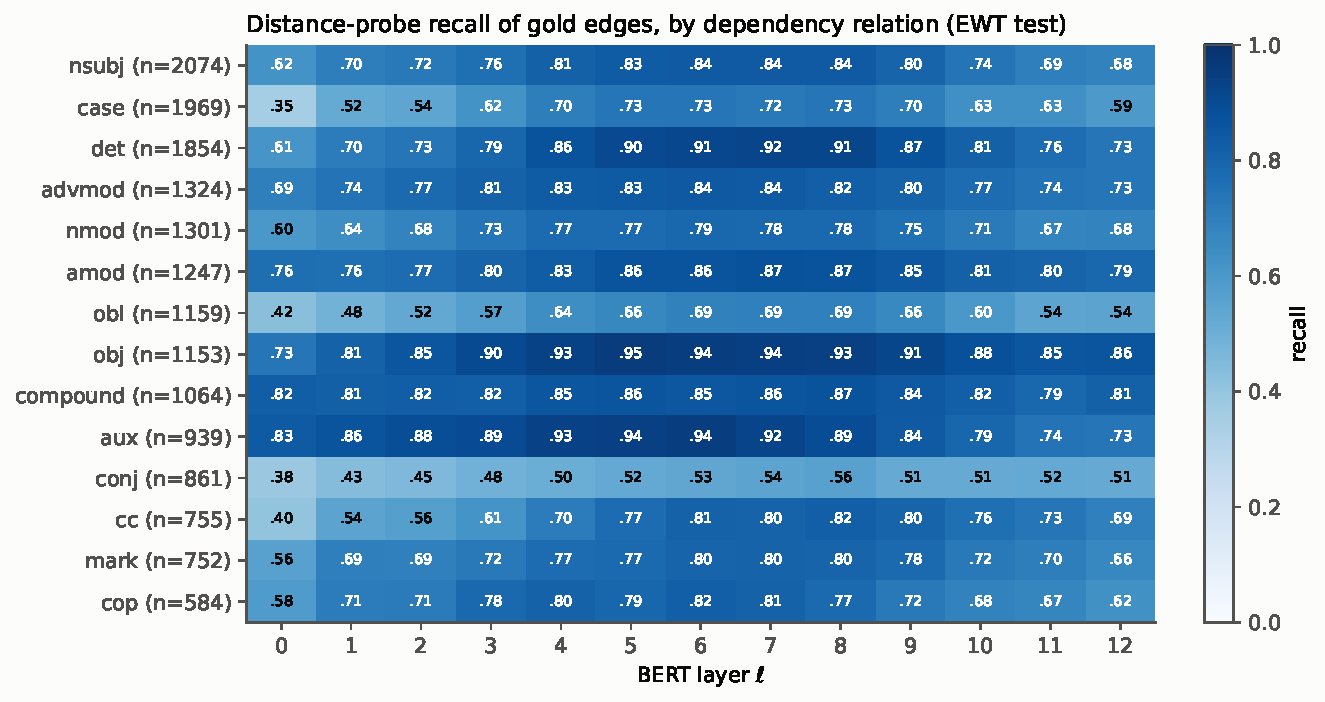
\includegraphics[width=0.82\textwidth]{relation_recall_heatmap.pdf}
\caption{T2 distance-probe recall per dependency relation and BERT layer (EWT test, dev-best rank per layer).}
\end{figure}
\begin{figure}[H]\centering
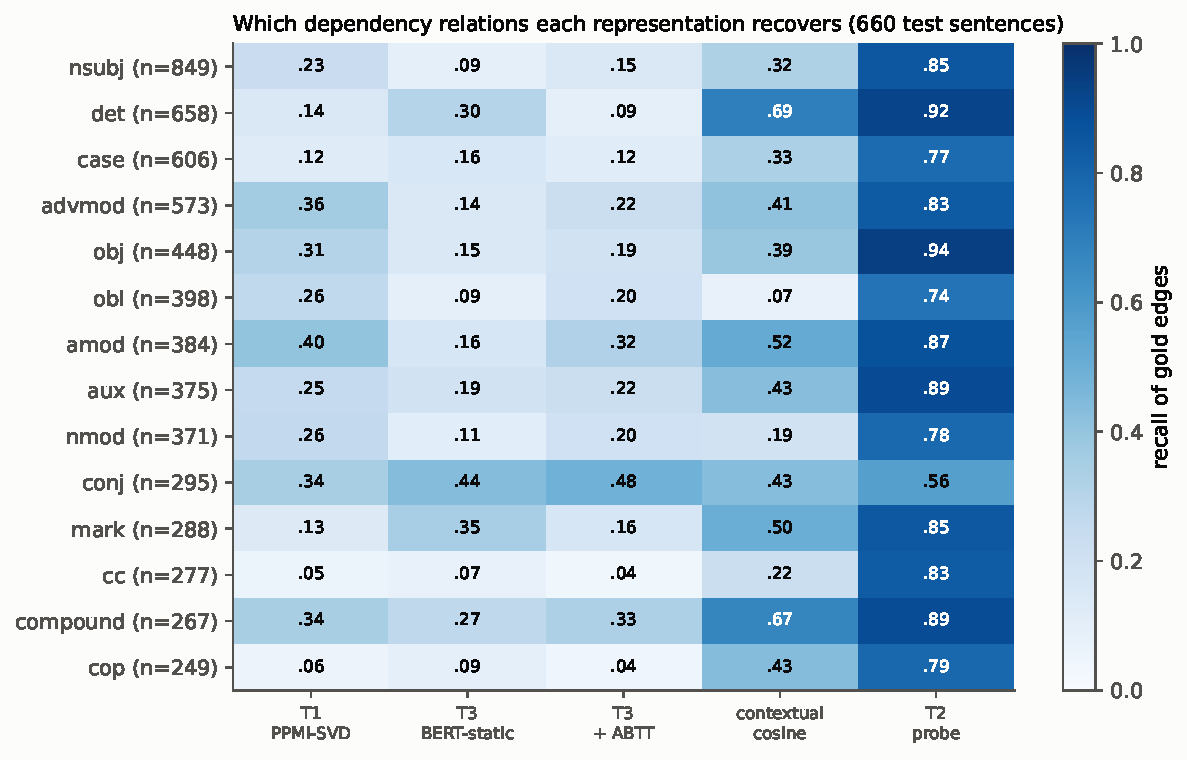
\includegraphics[width=0.72\textwidth]{ladder_relations.pdf}
\caption{Recall of gold edges per relation for each representation on the 660-sentence pool.}
\end{figure}
\begin{figure}[H]\centering
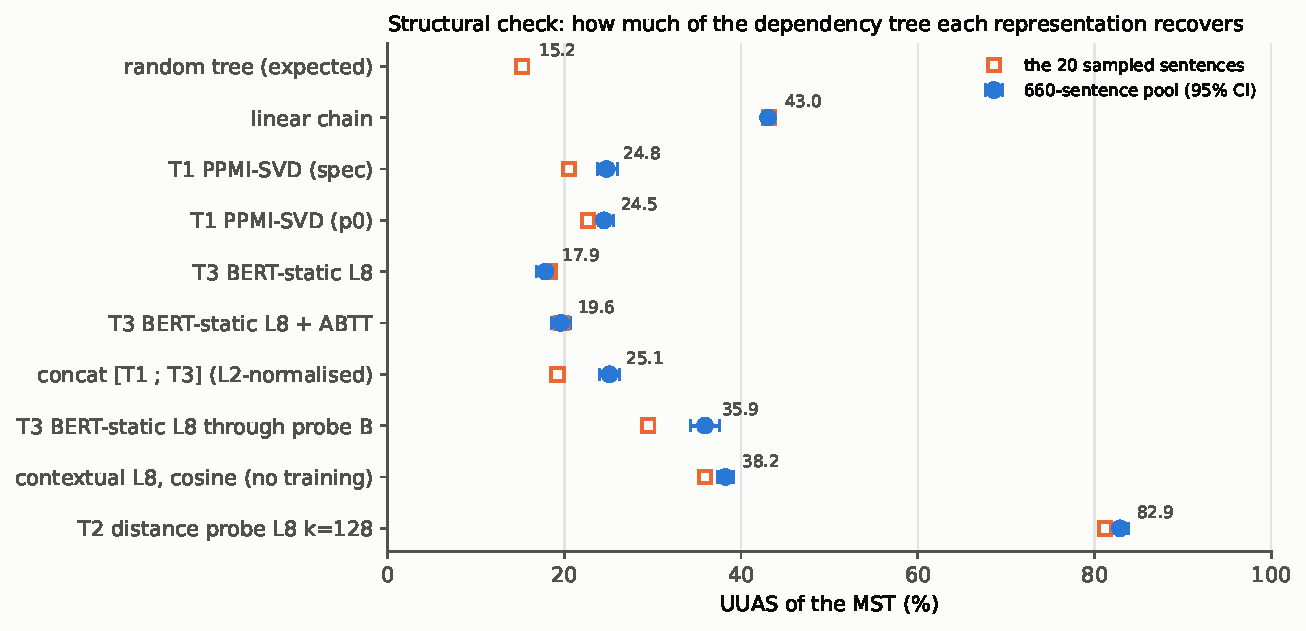
\includegraphics[width=0.80\textwidth]{ladder.pdf}
\caption{The diagnostic ladder (Table~\ref{tab:ladder}): pool UUAS with 95\% CI (filled) and the 20 sentences (open squares).}
\end{figure}
\begin{figure}[H]\centering
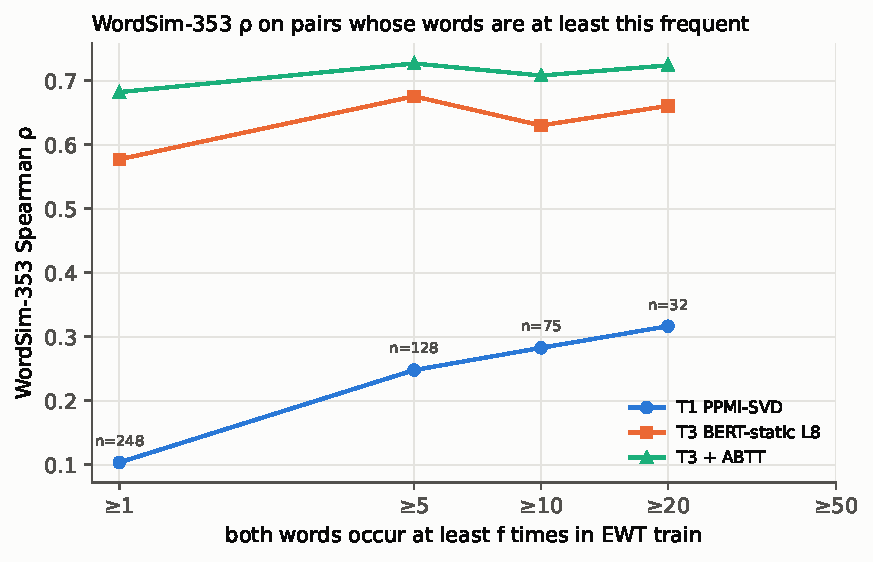
\includegraphics[width=0.62\textwidth]{ws_by_frequency.pdf}
\caption{WS-353 $\rho$ on pairs whose two words occur at least $f$ times in EWT train (n = number of pairs).}
\end{figure}
\begin{figure}[H]\centering
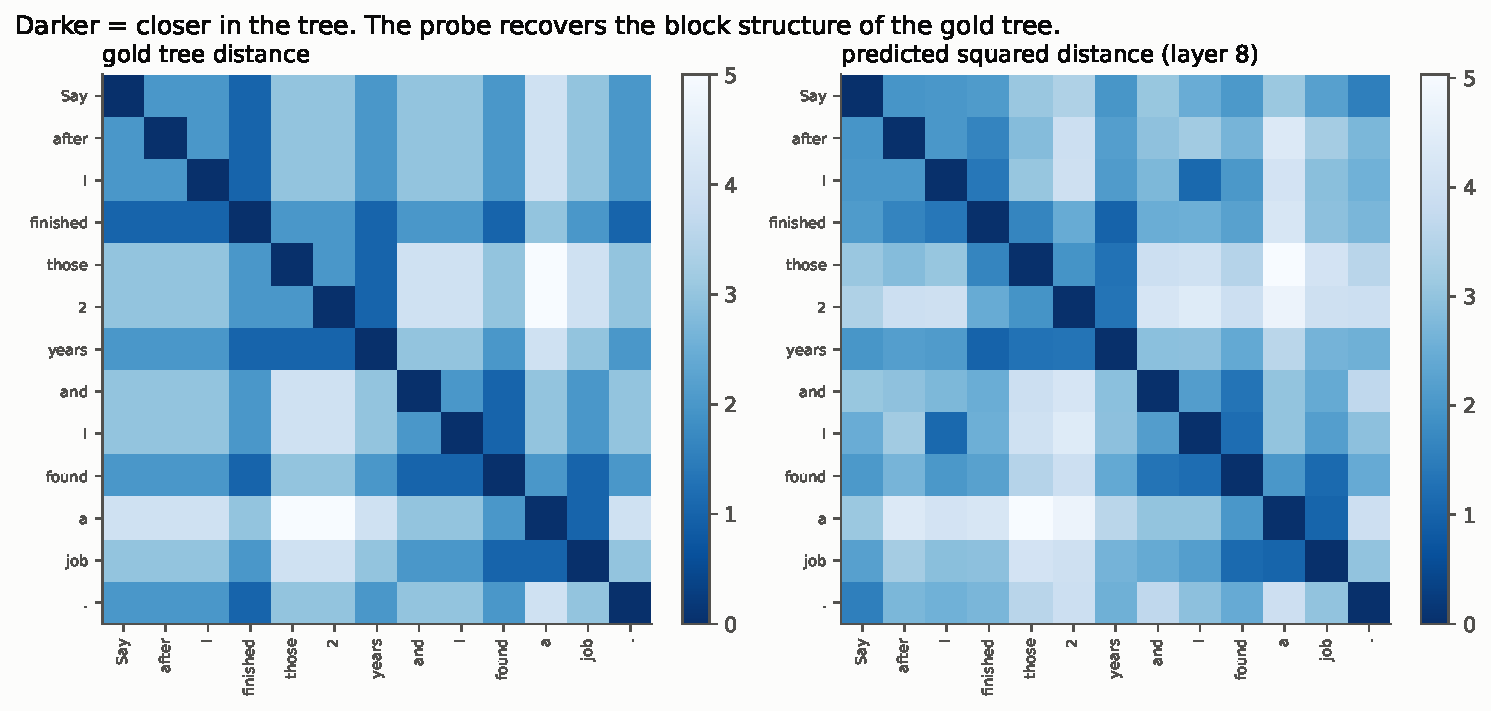
\includegraphics[width=0.95\textwidth]{distance_heatmap_typical.pdf}\\[2pt]
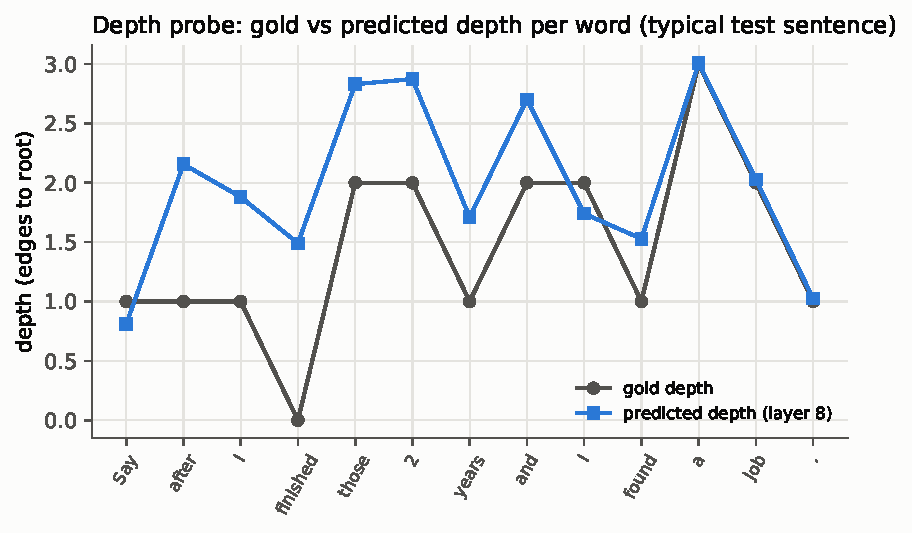
\includegraphics[width=0.70\textwidth]{depth_example_typical.pdf}
\caption{T2 on the median sentence: gold tree distances vs.\ predicted squared distances (top), gold vs.\ predicted depth (bottom).}
\end{figure}
\end{document}
